% !TEX encoding = UTF-8 Unicode
%% Template para dissertacao/tese na classe UFBAthesis
%% versao 1.0
%% (c) 2005 Paulo G. S. Fonseca
%% (c) 2012 Antonio Terceiro
%% (c) 2014 Christina von Flach
%% www.dcc.ufba.br/~flach/ufbathesis

%% Carrega a classe ufbathesis
%% Opcoes: * Idiomas
%%           pt   - portugues (padrao)
%%           en   - ingles
%%         * Tipo do Texto
%%           bsc  - para monografias de graduacao
%%           msc  - para dissertacoes de mestrado (padrao)
%%           qual - exame de qualificacao de mestrado
%%           prop - exame de qualificacao de doutorado
%%           phd  - para teses de doutorado
%%         * Media
%%           scr  - para versao eletronica (PDF) / consulte o guia do usuario
%%         * Estilo
%%           classic - estilo original a la TAOCP (deprecated) - apesar de deprecated, manter esse.
%%           std     - novo estilo a la CUP (padrao)
%%         * Paginacao
%%           oneside - para impressao em face unica
%%           twoside - para impressao em frente e verso (padrao)

% Atenção: Manter 'classic' na declaracao abaixo:
\documentclass[bsc, classic, a4paper]{ufbathesis}


%% Preambulo:
\usepackage[T1]{fontenc} %muda a codificação da fonte, tornando possível copiar textos com acentos no arquivo de saída, pdf.
\usepackage{lmodern} %usado com [T1], tornará as fontes com contornos de alta qualidade para as três famílias de fontes LaTeX.
\usepackage[utf8]{inputenc}
\usepackage{graphicx}
\usepackage[printonlyused,withpage]{acronym}
\usepackage{lipsum}

%%%%%%%%%%%%%%%%%%%%%
% Pacotes que inclui.
%%%%%%%%%%%%%%%%%%%%%

\usepackage{tabularx} %usado em tabelas para quebra de linha automática.
\usepackage{algpseudocode} %para pseudo-codigo.
\usepackage[portuguese,linesnumbered,ruled,vlined]{algorithm2e}
\usepackage{fancybox} %para caixa de texto.

% for comments while writing.
\usepackage{color}
\newcommand{\advisor}[1]{\textcolor{red}{\bf [Advisor]: #1}}
\newcommand{\you}[1]{\textcolor{blue}{[You]: #1}}

%%%%%%%%%%%%%%%%%%%%%

% Universidade
\university{Universidade Federal da Bahia}

% Endereco (cidade)
\address{Salvador}

% Instituto ou Centro Academico
\institute{Instituto de Matemática}

% Nome da biblioteca - usado na ficha catalografica
\library{Biblioteca Reitor Mac\^{e}do Costa}

% Colegiado de graduacao
\program{Bacharelado em Ci\^{e}ncia da Computa\c{c}\~{a}o}

% Area de titulacao
\majorfield{Ci\^{e}ncia da Computa\c{c}\~{a}o}

% Titulo da dissertacao
\title{Especificação e implementação de um mecanismo de monitoramento para um provedor de qualidade de serviço distribuído}

% Data da defesa
% e.g. \date{19 de fevereiro de 2013}
\date{16 de Dezembro de 2008}
% e.g. \defenseyear{2013}
\defenseyear{208}

% Autor
% e.g. \author{Jose da Silva}
\author{Hugo Vinicius Vaz Braga}

% Orientador(a)
% Opcao: [f] - para orientador do sexo feminino
% e.g. \adviser[f]{Profa. Dra. Maria Santos}
\adviser{Prof. Sérgio Gorender}

% Orientador(a)
% Opcao: [f] - para orientador do sexo feminino
% e.g. \coadviser{Prof. Dr. Pedro Pedreira}
% Comente se nao ha co-orientador
%\coadviser{Titulo e Nome Completo do CO-ORIENTADOR}

%% Inicio do documento
\begin{document}

\pgcompfrontpagebsc

%% Parte pre-textual
\frontmatter

\pgcomppresentationpage

%%%%%%%%%%%%%%%%%%%%%%%%%
% Ficha catalografica
%%%%%%%%%%%%%%%%%%%%%%%%%

\authorcitationname{Braga, Hugo Vinicius Vaz Braga} % e.g. Terceiro, Antonio Soares de Azevedo
\advisercitationname{Gorender, Sérgio} % e.g. Chavez, Christina von Flach Garcia
%\coadvisercitationname{Sobrenome, Nome do CO-ORIENTADOR} % e.g. Mendonca, Manoel Gomes de
\catalogtype{Monografia (Gradua\c{c}\~{a}o)} % e.g. ou ``Tese (Doutorado)''
%\catalogtype{Disserta\c{c}\~{a}o (Mestrado)} % e.g. ou ``Tese (Doutorado)''

%\catalogtopics{1. Primeira palavra-chave. 2. Segunda palavra-chave. 3. Terceira palavra-chave} % Listar palavras-chave do trabalho para a FICHA CATALOGRAFICA}, por exemplo, ``1. Complexidade Estrutural. 2. Qualidade de Software 3. Engenharia de Software''
%\catalogcdd{XXX.XX} % e.g.  XXX.XX (número nesse formato serah dado pela biblioteca)
%\catalogcdu{XXX.XX.XXX} % e.g.  XXX.XX.XXX (idem)
%\catalogingsheet

%%%%%%%%%%%%%%%%%%%%%
% Termo de aprovacaoo
%%%%%%%%%%%%%%%%%%%%%

\approvalsheet{Salvador, 16 de Dezembro de 2008}{
   \comittemember{Prof. Sérgio Gorender (Orientador)}{Universidade Federal da Bahia}
   \comittemember{Prof. Flávio Morais de Assis Silva}{Universidade Federal da Bahia}
   \comittemember{Prof. Raimundo José de Araújo Macêdo}{Universidade Federal da Bahia}
   % Para mestrado, apenas 3.
   % \comittemember{Prof. Dr. Professor 4}{Universidade HJKL}
   % \comittemember{Profa. Dra. Professora 5}{Universidade QWERTY}
}

%%%%%%%%%%%%%%%%%%%%%%%%%%%%%%%%%%%%%%%%
% Dedicatoria, Agradecimentos, Epigrafe
%%%%%%%%%%%%%%%%%%%%%%%%%%%%%%%%%%%%%%%%

% Comente para ocultar
%\begin{dedicatory}
%DIGITE A DEDICATORIA AQUI.
%\end{dedicatory}

% Agradecimentos
% Se preferir, crie um arquivo `a parte e o inclua via \include{}
%\acknowledgements
%DIGITE OS AGRADECIMENTOS AQUI.

% Epigrafe
%\begin{epigraph}[NOTA]{AUTOR}
%DIGITE AQUI A CITACAO.
%\end{epigraph}

%%%%%%%%%%%%%%%%%%%%%
% Resumo em Portugues
%%%%%%%%%%%%%%%%%%%%%

% !TEX encoding = UTF-8 Unicode
\resumo
%\begin{resumo}

	A capacidade de se adaptar dinamicamente às condições distintas de execução é uma questão muito importante quando se trata de sistemas distribuídos cuja Qualidade de Serviço (\textit{Quality of Service} - QoS) negociada nem sempre pode ser entregue entre os processos \cite{GMCR07}. Dado esta motivação, \cite{GMCR07} propuseram um modelo adaptativo de programação para sistemas distribuídos tolerantes à falhas. Para que este modelo possa funcionar corretamente, ele necessita obter informações sobre a QoS (além da execução de alguns outros serviços) provida aos canais de comunicação. Estas informações são obtidas através da interface padronizada denominada \textit{QoS Provider} (QoSP). Além da padronização, o \textit{QoS Provider} visa encapsular todos os detalhes a respeito das arquiteturas de QoS que estão sendo utilizadas. O QoSP pode ser resumido em dois grandes serviços: negociação e monitoração de QoS. Este trabalho visa desenvolver, especificar e implementar o mecanismo de monitoramento do QoSP. Este mecanismo corresponde ao serviço de monitoramento mencionado anteriormente. Este mecanismo engloba três funcionalidades: monitorar a QoS que está sendo provida a um canal de comunicação, verificar se há tráfego em um canal durante um intervalo de tempo e realizar um monitoramento automático.

\begin{keywords}
Sistemas distribuídos, QoS, monitoramento.
\end{keywords}

%\end{resumo}
%\resumo
%COLOQUE O RESUMO. Se preferir, crie um arquivo separado e o inclua via comando include.
%
%Para evitar problemas de formato neste template (de uso geral), usamos acentua\c{c}\~{a}o mostrada abaixo. 
%
%\begin{verbatim} 
%\c{c} \~{a} \'{a} \^{e} \'{\i}
%\end{verbatim} 
%
%N\~{a}o precisa fazer dessa forma, caso use pacotes adequados (latin1, etc.).
%
%% Palavras-chave do resumo em Portugues
%\begin{keywords}
%PALAVRAS-CHAVE.
%\end{keywords}

%%%%%%%%%%%%%%%%%%%
% Resumo em Ingles
%%%%%%%%%%%%%%%%%%%

\abstract
%\begin{spacing}{1.5}
%\parskip=6pt
Steiner trees are commonly used to model constraints in message multicasting. 
%Typically, a Steiner tree problem involves minimizing the total cost of the tree while satisfying additional constraints, such as bounded maximum node degree.
In this dissertation we address a problem called \emph{Directed k-Spanner with Minimum Degree Steiner Tree Problem} (DSMDStP). This problem
consists in, given a directed weighted graph $G(V,E)$, a \emph{source node} $s \in V$, 
a \emph{stretch factor} $k$ ($k \in \mathbb{R}^+$, $k \ge 1$) and a set of \emph{terminals} $T \subseteq V \setminus \lbrace s \rbrace$, 
finding an arborescence in which the cost (distance) between $s$ and each $t \in T$ 
is less than or equal to $k$ times the shortest distance between $s$ and $t$ in the original graph, 
while minimizing the maximum node out-degree. 
DSMDStP is not approximable sublogarithmically (unless $NP \subset DTIME(n^{\log \log{n}})$).
We describe an approximation algorithm that generates 
an arborescence with out-degree limited to $2\sqrt{|T|} + 2 + O(\log |T|) \cdot d^*$, where $d^*$ is the maximum degree in an optimum solution and 
the arborescence is a spanner with a root-stretch factor of 
$k \cdot \left(1 + \frac{max_{t\in T}\{dist(s,t,G)\}}{min_{t \in T}\{dist(s,t,G)\}}\right)$, 
where $dist(s,t,G)$ represents the shortest distance between $s$ and $t$ in $G$. 
%where $dist_{max} = max\{dist(s,t,G) | t \in T\}$ and $dist_{min} = min\{dist(s,t,G) | t \in T\}$. 
%Although our root-stretch factor is a function of $k$ and extreme terminal distance costs rather than only $k$, in simulations, the spanner guarantee 
%was really good. Actually, in average, the spanner constraint was satisfied. Besides this, the maximum out-degree was low compared to shortest path trees.
Although our root-stretch factor violates $k$, in our experiments the spanner constraint was satisfied or almost satisfied in average. 
Additionally, the resulted out-degree was low.
We also describe a heuristic which provides a root-stretch factor of $k \cdot (\lfloor\sqrt{|T|}\rfloor+2)$ but does
not provide a bound to the out-degree.
%We also describe a heuristic (called SIM) which does not provide a limit to the degree of nodes and has a root-stretch factor of $k \cdot (\sqrt{|T|}+2)$. 
%In our simulations, SIM exhibited interesting characteristics, having a stable behaviour for both degree and spanner guarantee, which contributes to scalability, 
%and also outperforming the other proposed algorithm regarding the degree.
In the experiments, the heuristic was shown to scale well in terms of the maximum degree achieved, and has always outperformed the other algorithms. The heuristic generated additionally a low spanner violation factor.
\begin{keywords}
Steiner tree, Directed Graph, Minimum Degree, Spanner, Approximation, Heuristic
\end{keywords}

%\end{spacing}

%\begin{otherlanguage*}{english}
%\abstract
%
%PUT THE ENGLISH ABSTRACT. If you'd prefer, create a separated file and include it with \texttt{include} command.
%COLOQUE O RESUMO EM INGL\^{E}S. Se preferir, crie um arquivo separado e o inclua via comando include.
%% Palavras-chave do resumo em Ingles
%\begin{keywords}
%KEYWORDS IN ENGLISH.
%PALAVRAS-CHAVE EM INGL\^{E}S.
%\end{keywords}
%\end{otherlanguage*}

%%%%%%%%%%%%%%%%%%%
% Sumario / Indice
%%%%%%%%%%%%%%%%%%%

% Comente para ocultar
\tableofcontents

% Lista de figuras
% Comente para ocultar
\listoffigures

% Lista de tabelas
% Comente para ocultar
%\listoftables

% Lista de Siglas
%\abbreviations
%% Sintaxe da lista de acordo com a documentação do pacote `acronym'
%% documentação: http://mirror.unl.edu/ctan/macros/latex/contrib/acronym/acronym.pdf
%\begin{acronym}[PGCOMP]
%    \acro{PGCOMP}{Programa de Pós-Graduação em Ciência da Computação}
%    \acro{CNPq}{Conselho Nacional de Desenvolvimento Científico e Tecnológico}
%\end{acronym}

%% Parte textual
\mainmatter

% !TEX encoding = UTF-8 Unicode
%\chapter{Introdução}% \label{sec:objetivo_geral}
\xchapter{Introdução}{}
\acresetall

	De acordo com \cite{GMCR07}, a capacidade de se adaptar dinamicamente às condições distintas de execução é uma questão muito importante quando se trata de sistemas distribuídos cuja Qualidade de Serviço (\textit{Quality of Service} - QoS) negociada nem sempre pode ser entregue entre os processos. Sistemas distribuídos são definidos como aqueles nos quais os componentes localizados em computadores interligados em rede se comunicam e coordenam suas ações apenas trocando mensagens \cite{COLDOKIN07}. Com relação à degradação da QoS, \cite{JTK00} afirma que esta é quase sempre inevitável e que a reserva de recursos não é suficiente para que a QoS seja sustentada. Levando em consideração este contexto, \cite{GMCR07} propuseram um modelo adaptativo de programação para sistemas distribuídos tolerantes à falhas.
	
	Este modelo (também conhecido como modelo HA - \textit{Hybrid and Adaptative}) é considerado híbrido, visto que é composto por partes assíncronas (nas quais não existem limites temporais para processamento e transferência de mensagens) e síncronas (nas quais existem limites temporais) mantidas por QoS, e adaptativo, visto que a QoS se altera e o modelo necessita se adaptar às condições de QoS. Para que o modelo HA possa funcionar corretamente, ele necessita obter informações sobre a QoS que está sendo provida a cada canal de comunicação.
	
	Tais informações são providas através do dispositivo de software denominado QoS Provider (QoSP). O QoSP corresponde a uma interface padronizada que cria e gerencia canais de comunicação com QoS. O QoSP não é uma arquitetura de QoS, mas sim um invólucro para um conjunto de arquiteturas para prover QoS. Dessa maneira, mesmo que o ambiente de comunicação seja alterado (novas arquiteturas de QoS sejam utilizadas), os processos que usufruem desta interface não sofrerão mudança alguma, visto que a interface do QoSP não muda. O QoSP deve se comunicar com as as arquiteturas de QoS existentes no ambiente para obter informações relativas a QoS de um canal.
	
	A interface do QoSP é definida através de cinco funções: criação de canal, cálculo de \textit{delay}, negociação de QoS, monitoração de QoS e verificação de canal. Apesar das cinco funções, o QoSP pode ser resumido em dois grandes serviços: negociação e monitoração de QoS. O serviço de monitoração engloba as funções de monitoração de QoS e de verificação de canal. A função de monitoração de QoS retorna a QoS que está sendo provida a um canal, enquanto que a função de verificação além de desempenhar tal funcionalidade ela verifica se há tráfego em um canal durante um determinado intervalo de tempo (estas funções serão detalhadas no capítulo \ref{cap:qos_provider}). Uma outra funcionalidade do serviço de monitoração é o monitoramento automático, que corresponde a um monitoramento que é executado mesmo quando não há uma solicitação explícita ao QoSP. 
	
	A monitoração de QoS é um mecanismo utilizado por outros componentes para obter um \textit{feedback} sobre o estado atual da QoS, para que medidas possam ser tomadas baseado neste \textit{feedback}. Isto se aplica bem ao modelo proposto HA, visto que para que o modelo HA possa afirmar que um determinado processo falhou, ele consultar o QoSP (mas especificadamente, o mecanismo de monitoramento). De acordo com \cite{ACH96}, mecanismos de monitoração de QoS são partes fundamentais de arquiteturas de QoS. O módulo (estou utilizando este termo intercambiável com mecanismo) de monitoração do QoSP não é um componente de arquitetura de QoS, mas se comporta como um para o QoSP, visto que é ele quem retorna ao QoS que está sendo provida ao longo dos componentes de software e hardware de um canal \cite{ACH96}. Logo justifica-se a adoção de princípios e de um modelo de sistema de monitoramento.
	
	Este trabalho visa desenvolver, especificar e implementar o mecanismo de monitoramento do QoS Provider, sendo que este último tem como base a arquitetura Diffserv e conta com um sistema operacional de tempo real instalado nos \textit{hosts}. O desenvolvimento deve ser baseado em um modelo e em princípios de sistema de monitoramento, além da utilização de protocolos que diminuam o \textit{overhead} da rede. A utilização de princípios assim como de protocolos que diminuam o \textit{overhead} visa não tornar o sistema de monitoramento um gargalo, mas sim um componente que auxilie a tomada de decisões. O desenvolvimento se dará através da especificação dos algoritmos que compõem o mecanismo de monitoramento assim como de um protocolo utilizado pelo mesmo. A especificação do sistema se dará através da modelagem do mesmo utilizando diagramas UML. Ao final da implementação, o sistema deverá ser testado.
% !TEX encoding = UTF-8 Unicode
%\chapter{QoS} 
\xchapter{QoS}{}
\label{cap:qos}
\acresetall
	QoS é o acrônimo para \textit{Quality of Service}, sendo um termo amplamente utilizado na literatura, mas em poucos artigos ele é definido. De acordo com \cite{GODERIS01}, QoS se refere a um serviço sendo oferecido onde um ou mais parâmetros de performance (isto é, vazão, atraso, perda e \textit{jitter}) podem ser quantificados. \cite{WANG01} define QoS como sendo "a capacidade de prover garantias de recursos e diferenciação de serviços em uma rede". Quando um canal de comunicação possui recursos reservados e algum nível de prioridade com relação a outros canais, podemos dizer que este canal possui uma QoS.	
	
\section{Arquiteturas de QoS}

	Diversas arquiteturas para prover QoS têm sido desenvolvidas nos últimos anos \cite{ACH96}. A motivação para a utilização de mecanismos de QoS, consequentemente para o desenvolvimento de arquiteturas de QoS, foi a necessidade de prover priorização e proteção a alguns fluxos de tráfegos \cite{GEBOSHIN03}, mas especificadamente aos tráfegos provindos das aplicações de tempo real, visto que estas necessitam de garantias temporais (previsibilidade). Este conjunto inclui os princípios que regem a construção de uma arquitetura genérica, a especificação da QoS que é necessária para capturar os requisitos da aplicação, e por último os mecanismos pelos quais os requisitos da aplicação serão atendidos. Basicamente os mecanismos podem ser divididos em dois tipos: provisão e controle/gerenciamento de QoS. Enquanto que o primeiro visa a reserva dos recursos, o outro visa a manutenção da QoS. Um dos componentes necessários para que esta manutenção ocorra corresponde ao monitoramento (não é o mesmo monitoramento do QoSP), pois é o mesmo que fornece o \textit{feedback} para saber se a QoS está sendo mantida. O módulo de monitoramento do QoSP deve se comunicar com o mecanismo de controle/gerenciamento das arquiteturas que estão sendo utilizadas no ambiente para conseguir obter a QoS que está sendo provida a um canal.
	
	Entre as diversas arquiteturas propostas na literatura, duas foram padronizadas pela IETF: os Serviços Integrados (\textit{Integrated Services} - \textit{IntServ}) e os Serviços Diferenciados (\textit{Differentiated Services} - \textit{Diffserv}). A seguir será apresentada de forma detalhada a arquitetura \textit{Diffserv}, visto que a mesma foi utilizada na implementação do QoSP.
	
\subsection{Diffserv}	

	Os Serviços Diferenciados \cite{BBCDWW98} baseiam-se na idéia de classes de comportamento, sendo que cada classe de comportamento define uma forma diferente de encaminhamento dos pacotes. Os pacotes pertencentes a diversos fluxos são agregados em classes e os pacotes da mesma classe são encaminhados na rede utilizando a mesma classe de comportamento. As reservas de recursos assim como o tratamento dado pelos roteadores (definido pelas classes de comportamento) aos pacotes é feito por classe, tornando o sistema escalável, visto que para um número grande de fluxos são configuradas poucas classes e, conseqüentemente, poucos estados são armazenados em cada roteador. Outra vantagem de se reservar recursos por classe é que raramente os recursos estarão ociosos, visto que frequentemente pelo menos um canal estará transmitindo algum dado. A maior parte do tráfego da Internet se comporta desta maneira, ou seja, nem todos os canais estarão transmitindo ao mesmo tempo.
	
	As classes de comportamento são chamadas de PHB (\textit{Per Hop Behavior}). As PHBs definem a forma como cada roteador irá encaminhar os pacotes para o outro roteador. Desta maneira, cada roteador deve possuir pré-configurado um conjunto de PHBs. Esta forma de encaminhamento se dá em termos dos recursos a serem utilizados e das propriedades do serviço que devem ser consideradas (como perdas, atraso, \textit{jitter}) \cite{GORENDER05}. Como podemos observar, a idéia do \textit{Diffserv} é oferecer níveis diferentes de serviço para os pacotes, ou seja, ele se baseia em um esquema de prioridade relativa \cite{XINI99}. O conjunto de fluxo de dados tratados da mesma forma (assinalados à mesma PHB) recebem o nome de Agregado de Comportamento (\textit{Behavior Aggregate}).
	
	Cada roteador identifica a classe de comportamento que será aplicada ao pacote através do \textit{DS Field}. Este corresponde a um campo do cabeçalho IP, e inclui seis bits que são utilizados pelo \textit{Diffserv} como um \textit{Codepoint} (\textit{DSCP}). Cada valor do \textit{DSCP} é mapeado para uma PHB em um roteador.

	Para que um determinado cliente possa receber Serviços Diferenciados do provedor de serviços (ISP), é necessário que seja estabelecido um Acordo de Ní­vel de Serviço (\textit{Service Level Agreement - SLA}) entre o cliente e o ISP. Este acordo informa o ní­vel de serviço assim como identifica as características do fluxo de dados que deverá receber o Serviço Diferenciado. O próprio cliente ou o ISP pode marcar o DSCP para configurar o serviço que será recebido pelo cliente.
	
	Um domí­nio \textit{Diffserv} (Figura \ref{fig:rede_diffserv}) é formado por roteadores (algumas literaturas chamam de nós) de dois tipos: roteadores de borda (também conhecidos como nós de fronteira) e de núcleo (também conhecidos como nós interiores) \cite{BBCDWW98}. Os roteadores de borda servem para interconectar domínios enquanto que os roteadores de núcleo apenas se conectam a outros roteadores do domínio. Os nós de fronteira implementam as funções de classificação, marcação, policiamento e condicionamento de tráfego, enquanto que os nós interiores apenas classificam, sendo que esta classificação é mais simples visto que ela é baseada apenas no DSCP, e encaminham pacotes. Esta estruturação da rede \textit{Diffserv} contribui para sua escalabilidade.
	
\begin{figure}
\centering
%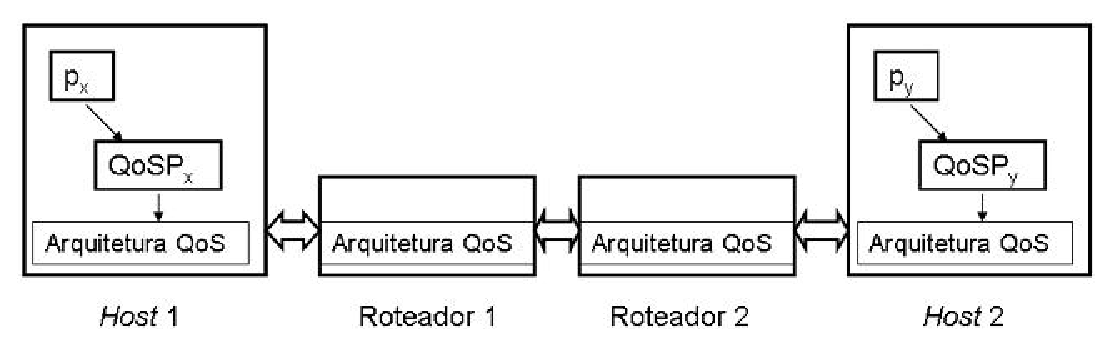
\includegraphics[width=0.3\textwidth]{qosp}
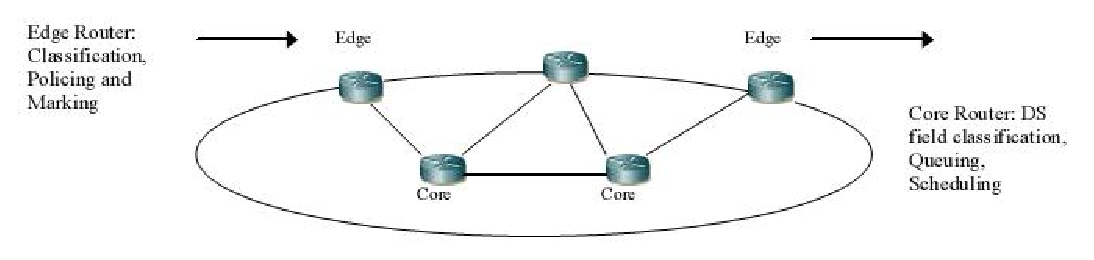
\includegraphics[scale=0.7]{rede_diffserv}
\caption{Rede Diffserv \cite{KFF03}}
\label{fig:rede_diffserv}
\end{figure}	
	
	Existem quatro PHBs padronizadas pelo IETF mas, para que o QoSP funcione (visto que os canais gerenciados pelo QoSP necessitam de dois tipos de serviços), apenas duas PHBs são necessárias e, consequentemente, serão abordadas: Padrão e o Serviço Expresso. Estes serviços caracterizam os níveis extremos de garantias, visto que enquanto o primeiro não possui garantia nenhuma, o segundo possui garantias suficientes para que o pacote sofra o menor atraso possível nos roteadores. 
	
\subsubsection{Padrão}

	A PHB Padrão especifica que os pacotes deverão receber o serviço melhor esforço (\textit{best-effort}). Neste caso, os pacotes que possuem tal serviço não têm prioridade e não possuem garantias de recursos. Este serviço será utilizado pelos canais de comunicação \textit{untimely}, que serão descritos no capítulo \ref{cap:qos_provider}.

\subsubsection{Serviço Expresso}	

	O Serviço Expresso (\textit{Expedited Forwarding} - EF), sendo também chamado em algumas bibliografias por serviço \textit{Premium}, basicamente visa garantir baixa latência e \textit{jitter}, além de uma largura de banda garantida. De forma intuitiva, para que o roteador forneça o Serviço Expresso basta que a taxa de saída dos pacotes seja maior ou igual a uma taxa de entrada previamente configurada \cite{BBCDWW98}. Com isso, caso os fluxos de dados não excedam a taxa de transmissão previamente configurada, praticamente estes pacotes não permanecerão em fila. Este serviço será utilizado pelos canais de comunicação \textit{timely}, descritos no capítulo \ref{cap:qos_provider}.
\section{Sistemas de monitoramento}	
	
	A monitoração de QoS é um mecanismo utilizado por outros componentes para obter um \textit{feedback} sobre o estado atual da QoS, para que medidas possam ser tomadas baseado neste \textit{feedback}. A reserva dos recursos não é suficiente para se obter QoS, visto que a degradação da mesma é inevitável \cite{JTK00}. De acordo com \cite{ACH96}, a monitoração da QoS é um componente essencial para o mecanismo de gerenciamento. Ela é responsável por descobrir o nível de QoS que está sendo provido por cada componente do serviço de comunicação para que se possa então verificar uma eventual degradação da qualidade de serviço fornecida. Quando a degradação é detectada, esta deve ser informada à aplicação e, neste caso, a aplicação poderá reagir de maneira adequada à perda da QoS, assumindo a perda no nível do serviço ou tentando renegociar uma nova QoS para o canal de comunicação. De acordo com \cite{ACH96}, o mecanismo de gerenciamento deve tentar resolver a perda da QoS antes de informar à aplicação sobre a degradação. O módulo de monitoração do QoSP deve apenas verificar e informar a QoS que está sendo provida ao canal, não sendo necessário resolver uma possível perda.
	
	Mesmo o módulo de monitoração do QoSP não sendo um componente de um arquitetura de QoS, ele se comporta como um para o QoSP, visto que ele é responsável por descobrir o nível de QoS que está sendo provido por cada arquitetura de QoS utilizada. Sendo assim, é importante que modelos e princípios de um sistema de monitoramento sejam utilizados.
	
\subsection{Princípios} %\label{subsub: principios}

	De acordo com \cite{ATIPPEB02}, a escalabilidade nas redes IP com QoS está ligada a três fatores: tamanho da topologia da rede, número e granularidade das classes de serviço suportadas na rede e o número de clientes que utilizam os serviços. Um sistema de monitoramento é considerado escalável se o mesmo consegue monitorar de forma eficiente uma grande rede com vários serviços e uma grande quantidade de clientes. Além disso, o sistema de monitoramento deve realizar as seguintes tarefas: coletar, agregar e analisar dados, além de prover um \textit{feedback} sobre a QoS atual. Ainda de acordo com \cite{ATIPPEB02}, para que o sistema de monitoramento seja escalável, é preciso que o mesmo siga os  princípios descritos abaixo.

\begin{enumerate}

\item Definir granularidade do processo de monitoramento
	
	Os algoritmos de monitoramento devem operar no nível do agregado e não no nível do pacote, visto que coletar dados no nível de pacote é  extremamente custoso e não escalável. No Diffserv, estas estatísticas seriam coletadas por PHB.
	
\item Distribuir o sistema coletor de dados
	
	Para que o sistema coletor de dados não gere um \textit{overhead} grande na rede, ele deve ser distribuído, preferencialmente um agente coletor por cada roteador e o mais próximo possível do mesmo.
	
\item Minimizar o \textit{overhead} da transmissão das medições através do processamento dos dados brutos próximo às fontes

	Assim como o sistema de coleta de dados, o processamento e sumarização dos dados também deve ser distribuído para que o sistema seja escalável. Além do mais, o sistema de monitoração pode adotar a política de notificação de eventos quando certos limiares são ultrapassados. A notificação é utilizada para evitar a sobrecarga da rede com interações desnecessárias entre componentes requisitando informações de monitoramento.
	
\item Utilizar medições por agregado em combinação com medições por canal

	Vários fluxos de dados possuem requisitos diferentes e por isso devem ser monitorados de forma diferente. Mas monitorar os canais de forma diferente torna o sistema complexo. Além disso, vários canais de comunicação passam pelo mesmo caminho na rede, conseqüentemente as medições feitas para um canal podem ser utilizadas para os outros canais, colaborando para a escalabilidade do sistema. Dessa forma deve-se optar por uma medição por agregado e, quando isso não for possível devido a requisitos diferentes ou caminhos diferentes pelos quais os canais passam, utiliza-se a medição por canal.

\end{enumerate}	

\subsection{Modelo de monitoramento de QoS} %\label{subsub: modelo}

	De acordo com \cite{JTK00}, os mecanismos de monitoramento podem ser divididos em duas categorias, baseado na informação de QoS que pode ser obtida através deles: monitoração de QoS fim-a-fim e a monitoração distribuída de QoS. Na monitoração fim-a-fim, apenas a QoS fim-a-fim de um canal de comunicação é monitorada. Neste caso, a degradação da QoS consegue ser detectada, mas o componente que está causando tal degradação não. Na abordagem distribuída, a QoS que está sendo provida por cada elemento ao longo do canal é monitorada, permitindo saber quais são os elementos que estão causando a degradação. Enquanto que na abordagem fim-a-fim as informações de monitoramento são coletadas nos sistemas fins, ou seja nos \textit{hosts}, na abordagem distribuída estas informações são colhidas dos monitores relevantes, ou seja, dos elementos que estão monitorando os roteadores que fazem parte de um determinado canal. A abordagem distribuída além de contribuir para a escalabilidade permite que medidas de correção sejam tomadas, visto que o problema pode ser isolado. O modelo de monitoramento adotado em \cite{JTK00} (Figura \ref{fig:modelo}) é semelhante ao modelo tradicional de sistema de monitoramento apresentado em \cite{STALL96}, sendo dividido nos seguintes componentes:

\begin{figure}
\centering
%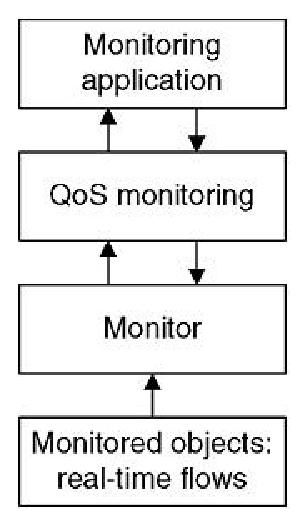
\includegraphics[width=0.3\textwidth]{modelo}
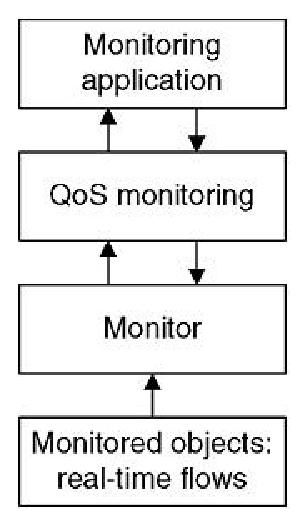
\includegraphics[scale=0.7]{modelo}
\caption{Modelo de monitoramento de QoS \cite{JTK00}}
\label{fig:modelo}
\end{figure}

\textbf{Monitoring application:} Este componente provê a interface do sistema de monitoramento com o usuário (ou um outro cliente interessado na informação de monitoramento, como o detector de defeitos). Recolhe (agrega) as informações colhidas pelos \textit{monitores} (o componente \textit{Monitor}), analisa estas informações e provê os resultados da análise para o usuário. Estes resultados correspondem à QoS que está sendo provida ao canal de comunicação.

\textbf{QoS monitoring:} Este componente não existe no modelo tradicional. Este componente provê mecanismos para permitir que \textit{Monitoring application} recupere a informação dos \textit{monitores} relevantes, ou seja, aqueles que monitoram os roteadores que fazem parte do canal de comunicação em questão. A QoS do canal é derivada a partir das informações capturadas pelos \textit{monitores}.

\textbf{Monitor:} É responsável por colher e armazenar as informações provenientes dos roteadores. Estas informações são comunicadas ao \textit{Monitoring application}.

\textbf{Monitored objects:} Estes objetos correspondem aos atributos e atividades que devem ser monitoradas na rede. Estes objetos equivalem a contadores dos fluxos de tempo real monitorados.

	Como foi explicado anteriormente, o sistema de monitoramento desempenha um conjunto de funções básicas. Estas funções podem ser mapeadas para o modelo descrito acima da seguinte maneira: a função de coletar os dados fica à cargo de \textit{Monitor}, enquanto que as funções de agregação e análise dos dados, além do \textit{feedback} provido contendo a QoS do canal são de responsabilidade de \textit{Monitoring application}.

\subsection{Colhendo informações de QoS}
	Os sistemas de monitoramento precisam se comunicar com os elementos de rede (como os roteadores) para colher informações de QoS. Algumas vezes essas interações são necessárias para que informações mais detalhadas sobre o estado da QoS que está sendo provida pelos elementos sejam capturadas. O protocolo SNMP é utilizado para gerenciar os elementos de rede, sendo descrito a seguir.
	
\subsubsection{SNMP}

	O SNMP (\textit{Simple Network Management Protocol}) foi concebido para monitorar os nós (\textit{hosts}, \textit{switches}, roteadores, etc) na Internet \cite{CFSD90}. Ele é formado por três componentes: o agente, o gerente (conhecido também como sistema de gerenciamento) e os dispositivos gerenciados (\textit{hosts}, roteadores, etc). Os agentes são elementos de software instalados nos dispositivos gerenciados cuja função principal é enviar informações relativas aos dispositivos para os gerentes.
	
	Todas as informações gerenciáveis são definidas através de variáveis nos dispositivos gerenciados. Estas variáveis contém valores que são lidos (quando o gerente solicita ao agente uma operação de leitura) ou atualizados (quando o gerente solicita ao agente uma operação de escrita). Essas informações gerenciáveis podem ser: número IP, quantidade de pacotes descartados, tamanho de filas, largura de banda reservada para classes, dentre inúmeras outras. Estas variáveis são estruturadas hierarquicamente (como numa árvore) na MIB.
	
	 Uma \textit{Management Information Base} (MIB) contém a definição dos objetos gerenciáveis. Os objetos gerenciáveis são conhecidos como objetos MIB, e são formados por várias instâncias de objeto. Por exemplo, um número de interface em um roteador é um objeto MIB e, sabendo que um roteador é formado por várias interfaces, o número de uma interface específica seria uma instância de objeto. Cada instância de objeto é identificada por um OID (\textit{object identifier}). Cada instância de objeto corresponde à uma variável citada anteriormente.
% !TEX encoding = UTF-8 Unicode
%\chapter{QoS Provider}
\xchapter{QoS Provider}{}
\label{cap:qos_provider}
\acresetall

	Como foi descrito na introdução, para que o modelo HA funcione corretamente, ele necessita obter informações sobre a QoS que está sendo provida aos canais de comunicação. Essas informações são obtidas através da infraestrutura de comunicação e gerenciamento de recursos para sistemas distribuídos com QoS denominada \textit{QoS Provider} (QoSP). O objetivo desta infraestrutura é fornecer e gerenciar canais de comunicação providos com QoS \cite{GORENDER05}. Para isso, o QoSP é definido através de uma interface padronizada que fornece um conjunto fixo de serviços, descritos nas próximas seções. Através desta padronização, o QoSP visa tornar o modelo citado anteriormente portável para diversas arquiteturas de QoS. Ele pode ser visto como um invólucro para um conjunto de arquiteturas de QoS, sendo assim deve se comunicar com as arquiteturas existentes no ambiente para obter as informações relativas a QoS de um canal de comunicação.
	
	Considera-se que um sistema distribuído é composto por um conjunto de processos, os quais executam em um ou mais \textit{hosts}. Este conjunto é representado por $\Pi = \lbrace p_{1}, p_{2}, ..., p_{n} \rbrace$, sendo $p_{x}$ um processo qualquer deste conjunto e \textit{n} o número de processos pertencentes ao sistema. Um canal de comunicação estabelecido entre os processos $p_{x}$ e $p_{y}$ é identificado por $c_{x/y}$ e $\Gamma$ é o conjunto de todos os canais de comunicação estabelecidos.

\section{Ambiente de execução} %canais de comunicaçao, serviços isocronos e nao-isocronos, timely e untimely

	Os canais de comunicação aqui utilizados são definidos como confiáveis e são providos com diferentes níveis de QoS. Canais confiáveis são aqueles que não perdem, não duplicam e nem alteram as mensagens. Os canais de comunicação são estabelecidos entre dois processos localizados em \textit{hosts} diferentes, definidos através de uma rota estabelecida em uma rede de computadores, sendo que esta rota é formada por um ou mais roteadores.
	
	As arquiteturas de QoS padronizaram várias classes de serviço (no capítulo \ref{cap:qos} foram descritas duas classes de serviço para a arquitetura Diffserv). Baseado nas diversas classes de serviço padronizadas pelas diversas arquiteturas de QoS, \cite{GORENDER05} definiu duas classes de serviço: Serviços Isócronos e Serviços Não Isócronos. Os Serviços Isócronos são serviços de comunicação que possuem limites temporais determinados para o processamento e transferência das mensagens. Os serviços Não Isócronos não fornecem nenhum limite temporal tanto para o processamento como para a tranferência das mensagens. Os canais de comunicação que	utilizam os Serviços Isócronos são denominados canais \textit{timely} enquanto que os canais que utilizam os Serviços Não Isócronos são denominados canais \textit{untimely}.
	
\section{Arquitetura do QoS Provider}

	O QoS Provider executa distribuído, sendo que existe um módulo do QoSP para cada \textit{host} do sistema. Os módulos do QoSP necessitam trocar mensagens entre si e com os roteadores para que as funções definidas na sua interface possam funcionar corretamente. Quando um processo $p_{x}$ necessita criar canais de comunicação com QoS e acessar informações de QoS dos mesmos, ele faz isso através do módulo $QoSP_{x}$, sendo $QoSP_{x}$ o módulo do QoSP localizado no mesmo \textit{host} de $p_{x}$.
	
	Para que o QoSP possa funcionar corretamente, os canais de comunicação utilizados pelos módulos do QoSP também necessitam utilizar os serviços das arquiteturas de QoS, discutidos no tópico anterior. Isto se faz necessário visto que os módulos do QoSP precisam se comunicar para realizar suas tarefas e, para que as informações providas pelos mesmos sejam confiáveis, eles também necessitam de reservas de recursos. Para isso, o QoSP também utilizará os serviços da arquitetura \textit{Diffserv} e um sistema operacional de tempo real instalado nos \textit{hosts} (o sistema operacional de tempo real utilizado na implementação do QoSP e pelos processos clientes será apresentado no capítulo \ref{cap:tempo_real}).
	
\section{Interface do QoS Provider}

	De acordo com \cite{GORENDER05}, a interface do QoSP pode ser definida através das seguintes funções:
	
\begin{itemize}
\item \textit{CreateChannel}$(p_{x},p_{y}):\Pi^{2}\rightarrow\Gamma$
	
	Cria um canal de comunicação entre os processos $p_{x}$ e $p_{y}$, retornando o novo canal, identificado por $c_{x/y}$, pertencente ao conjunto $\Gamma$. Todo canal deve ser criado como \textit{untimely}. As informações referentes ao canal, como a sua QoS, devem ser armazenadas pelo QoSP.
	
\item \textit{DefineQoS}$(p_{x}, p_{y}, \textit{qos}):\Pi^{2}\times\lbrace\textit{timely},\textit{untimely}\rbrace\rightarrow\lbrace\textit{timely},\textit{untimely}\rbrace$
	
	Altera a QoS provida ao canal de comunicação $c_{x/y}$ entre \textit{timely} e \textit{untimely}. Caso a solicitação seja de \textit{untimely} para \textit{timely}, um processo de admissão deverá ser executado.
	
\item \textit{Delay}$(p_{x}, p_{y}):\Pi^{2}\rightarrow N^{+}$
	
	Calcular um limite máximo, caso o canal seja \textit{timely}, ou um limite probabilístico, caso o canal seja \textit{untimely}, para o tempo de ida e volta (RTT maior ou igual ao \textit{Round trip time}) de transferência de uma mensagem entre os processos $p_{x}$ e $p_{y}$.
	
\item \textit{QoS}$(p_{x}, p_{y}):\Pi^{2}\rightarrow\lbrace\textit{timely},\textit{untimely}\rbrace$
	
	Verificar a QoS que está sendo provida ao canal de comunicação $c_{x/y}$, retornando a classe de serviço (\textit{timely} ou \textit{untimely}) que está sendo provida ao mesmo. Quando a QoS de um canal for alterada de \textit{timely} para \textit{untimely}, os processos ligados ao canal devem ser informados de tal degradação.
	
\item \textit{VerifyChannel}$(c_{x/y}):\Gamma\rightarrow\lbrace\textit{timely},\textit{untimely}\rbrace$
	
	Assim como a função \textit{QoS}, esta função tem como objetivo verificar a QoS que está sendo provida a um canal de comunicação ($c_{x/y}$). Uma das diferenças com relação à função \textit{QoS} é que ela é chamada por um processo $p_{i}$, sendo $p_{i} \neq p_{x}$ e $p_{i} \neq p_{y}$ (mais detalhes sobre esta função será explicado na próxima seção). A outra diferença é que esta função além de verificar a QoS que está sendo provida ao canal, através da chamada da função \textit{QoS} por exemplo, verifica a existência de tráfego no canal $c_{x/y}$. A não existência de tráfego durante um certo intervalo de tempo no canal (sendo que este intervalo de tempo é estabelecido pelo modelo HA) faz com que a QoS do canal seja alterada para \textit{untimely}.

\end{itemize}

	Além das funções citadas acima, cada módulo do QoSP deve monitorar de forma automática todos os canais \textit{timely} gerenciados pelo mesmo, com o intuito de verificar se estes canais continuam sendo providos com serviço Isócrono. Esta monitoração deve ocorrer periodicamente e, caso seja detectado que a QoS de um canal alterou de \textit{timely} para \textit{untimely}, os processos ligados ao canal devem ser notificados de tal degradação.
		
\section{O mecanismo de monitoramento do QoSP}

	Como já foi dito na introdução, apesar da interface do QoSP ser definida através de cinco funções (descritas na seção anterior), ela pode ser resumida em dois grandes serviços: negociação e monitoração. Enquanto que o serviço de negociação pode ser considerado um mecanismo estático de QoS, o serviço de monitoração pode ser considerado um mecanismo dinâmico \cite{ACH96}. Enquanto o serviço de negociação visa basicamente a reserva dos recursos, o serviço de monitoração visa garantir que os processos aplicativos tenham um \textit{feedback}, o quanto mais cedo possível, sobre o serviço que está sendo provido aos seus canais de comunicação. Este \textit{feedback} pode ser obtido através de uma solicitação explícita por parte dos processos aplicativos, ou através de uma notificação provida pelo mecanismo de monitoramento aos processos aplicativos, quando há uma alteração de QoS dos seus canais.
	
	Baseado no que foi descrito acima, o mecanismo de monitoramento do QoSP, também conhecido como \textit{QoS Provider Monitoring} (QoSPM), engloba as seguintes funções da interface do QoSP: \textit{QoS} e \textit{VerifyChannel}. Ambas procuram fornecer um \textit{feedback} sobre a QoS atual do canal para que medidas possam ser tomadas. Além destas funções, o monitoramento automático também faz parte do QoSPM, sendo ele equivalente à chamada periódica da função \textit{QoS}.
	
	A função \textit{QoS} executa a verificação da QoS de um canal $c_{x/y}$, sendo $p_{x}$ o solicitante da verificação. Esta é efetuada através do envio de mensagens de verificação a todos os roteadores pertencentes a $c_{x/y}$ e ao módulo $QoSP_{y}$, além do estabelecimento de \textit{timeouts} para a recepção das respostas. O módulo do QoSP (mas especificadamente o $QoSP_{x}$) fica aguardando as respostas de todas as mensagens enviadas. Se todas as mensagens chegam antes de \textit{timeout} (calculado através da função \textit{Delay}) e indicam que o serviço Isócrono está sendo provido, assume-se que a QoS do canal é \textit{timely}. Em qualquer outra situação, assume-se que a QoS do canal é \textit{untimely}. Caso a função \textit{QoS} mostre que a QoS do canal foi alterada de \textit{timely} para \textit{untimely}, os processos ligados ao canal devem ser informados de tal alteração.
	
	A função \textit{VerifyChannel} também verifica a QoS de um canal $c_{x/y}$, sendo $p_{i}$ o processo solicitante da verificação. Como $p_{i} \neq p_{x}$ e $p_{i} \neq p_{y}$, caso $p_{i}$ não  esteja no mesmo \textit{host} de $p_{x}$ nem de $p_{y}$, o módulo $QoSP_{i}$ deverá solicitar uma verificação remota ou ao módulo $QoSP_{x}$ ou ao módulo $QoSP_{y}$. Independente do módulo que execute a verificação, ela é efetuada da seguinte maneira: executa-se a função \textit{QoS} e, caso o retorno da função seja \textit{untimely}, o retorno da função \textit{VerifyChannel} também será \textit{untimely}. Caso contrário (o retorno de \textit{QoS} seja \textit{timely}), será verificado se os processos $p_{x}$ e $p_{y}$ trocam mensagens nos próximos $\Delta{t}$ (sendo $\Delta{t}$ estabelecido pelo modelo HA). Caso ocorra troca de mensagens neste intervalo de tempo, o retorno da função \textit{VerifyChannel} será \textit{timely}, caso contrário será \textit{untimely}.
	
	Assim como os processos aplicativos interagem com o QoSPM, o módulo de negociação do QoSP também precisa interagir com o QoSPM. Quando a QoS de uma canal é alterada (através da função \textit{DefineQoS}), esta informação precisa ser passada ao QoSPM.
% !TEX encoding = UTF-8 Unicode
%\chapter{Sistema Operacional de Tempo Real}
\xchapter{Sistema Operacional de Tempo Real}{}
\label{cap:tempo_real}
\acresetall
	
	De acordo com \cite{VERGO01}, sistemas de tempo real podem ser definidos como sendo aqueles cuja progressão é especificada em termos dos requisitos de \textit{timeliness} ditados pelo ambiente. \textit{timeliness} é uma propriedade que especifica que um determinado predicado $ \rho $ será verdadeiro em dado instante de tempo. A partir desta definição, podemos observar que sistemas de tempo real estão relacionados com previsibilidade. Esta previsibilidade é necessária para que tanto os canais \textit{timely} (descritos no capítulo \ref{cap:qos_provider}) possam ser providos como também para que estes possam ser gerenciados da maneira correta pelo QoSP.
	
	Nas seções seguintes serão descritas as abordagens utilizadas para se desenvolver os sistemas operacionais de tempo real (\textit{Real-time Operating Systems} - RTOS), sendo que nas duas últimas seções serão descritos os dois \textit{frameworks} de tempo real utilizados pelo QoSP.
	
\section{Abordagens de RTOS}

	De acordo com \cite{YOBA97}, existem três abordagens principais para construir um sistema operacional de tempo real: construir um sistema operacional específico para tempo real, adicionar suporte a tempo real em um sistema operacional de propósito geral (SOPG) e, por último, utilizar um sistema operacional de tempo real juntamente com um de propósito geral em um mesmo computador. A primeira abordagem é pouco utilizada visto que a maioria dos drivers são desenvolvidos para sistemas operacionais de uso geral, limitando a utilização destes sistemas operacionais específicos. As duas outras abordagens serão discutidas a seguir. Apesar destas abordagens não serem específicas para um determinado projeto, nos projetos pesquisados, estas são desenvolvidas utilizando como base o Linux. Isto se explica devido ao fato do Linux ser um sistema operacional livre, com o código fonte disponível. Sendo assim, em algumas situações a expressão \textit{sistema operacional de propósito geral} e a palavra \textit{Linux} serão utilizados de forma intercambiável.
	
\subsection{SOPG com suporte de tempo real}

	Esta abordagem, também conhecida como \textit{Preemption Improvement}, visa diminuir o tamanho das seções de código não preemptável, além de transformar o \textit{kernel} em versão totalmente preemptável (preemptável se refere à capacidade do sistema operacional de liberar um recurso em posse de um processo). Com isso, tratadores de interrupção e seções críticas passam a ser preemptáveis. O menor tempo de latência de escalonamento (sendo que esta latência se refere ao tempo decorrido entre a ocorrência de um evento externo e o início de execução da tarefa) está relacionado diretamente com o maior trecho de código não preemptável, por isso, limitar o tamanho deste trecho é importante para que restrições de tempo (\textit{soft} ou \textit{hard}) possam ser alcançadas. O \textit{patch} (arquivo que contém um código a ser adicionado em um outro código fonte de programa visando corrigir um \textit{bug} ou adicionar alguma(s) funcionalidade(s)) de preempção de tempo real (PREEMPT\_RT) \cite{MCKENNEY05} para o \textit{kernel} do Linux desenvolvido por Ingo Molnar utiliza esta abordagem.
	
\subsection{SOPG e RTOS compartilhando o mesmo computador}

	Nesta abordagem, também conhecida como \textit{Interrupt abstraction}, um \textit{kernel} de tempo real executa independente do \textit{kernel} do linux. A idéia é que os dois ambientes (Linux e RTOS) executem lado a lado, utilizando um \textit{micro-kernel} que gerencia as interrupções geradas pelo hardware \cite{GERUM04}. O \textit{kernel} do linux passa a ter prioridade mais baixa, comparada com os processos gerenciados pelo RTOS. A expressão \textit{Interrupt abstraction}  se deve ao fato de que o \textit{micro-kernel} cria uma abstração de interrupção (também conhecida como cano de interrupção), onde as interrupções chegam primeiro para o ambiente de tempo real e, caso não pertençam a este ambiente, passam para o Linux. Os principais projetos que utilizam esta abordagem são: Real-Time Linux \cite{YOBA97}, RTAI \cite{RTAI08} e Xenomai \cite{GERUM04}.

\section{Xenomai}

	O Xenomai é um \textit{framework} de desenvolvimento de tempo real, que executa de forma cooperativa com o \textit{kernel} do Linux, com o intuito de prover aos programas aplicativos suporte de tempo real rígido \cite{XENOMAI08}. De acordo com \cite{GERUM04}, o objetivo inicial do Xenomai é permitir aos desenvolvedores portar seus programas de tempo real, que executam em um RTOS específico, para o ambiente GNU/Linux sem a necessidade de reescrever suas aplicações completamente.
	
	A portabilidade dos programas aplicativos, citada anteriormente, é possível graças ao fato do Xenomai ser agnóstico com relação à API que está sendo utilizada, visto que ele permite que os processos de tempo real utilizem diversas APIs para se comunicar com o seu núcleo. O Xenomai é formado por um núcleo que exporta um conjunto genérico de serviços. Estes serviços são agrupados em uma interface de alto nível, permitindo a implementação de vários módulos que emulam diversos RTOS, tais como VxWorks, pSOS, uITRON, VRTX, entre outros (Figura \ref{fig:xenomai_skins}). Este conjunto de serviços também foi utilizado para implementar uma API nativa e uma API em conformidade com o padrão POSIX.
	
\begin{figure}
\centering
%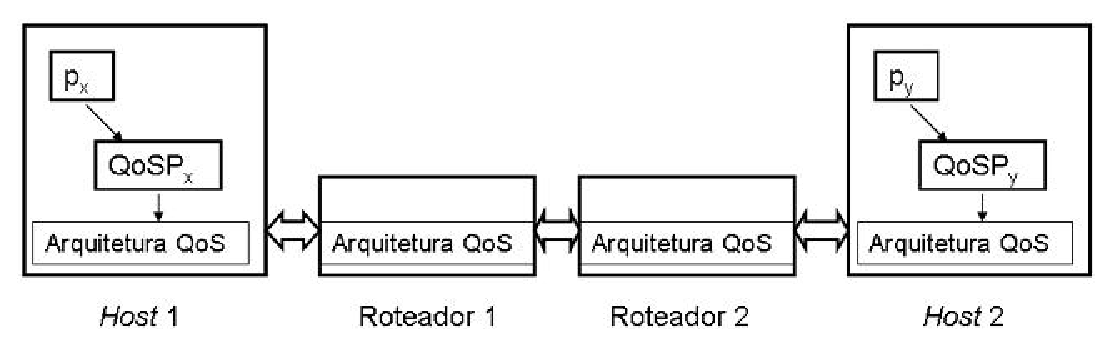
\includegraphics[width=0.3\textwidth]{qosp}
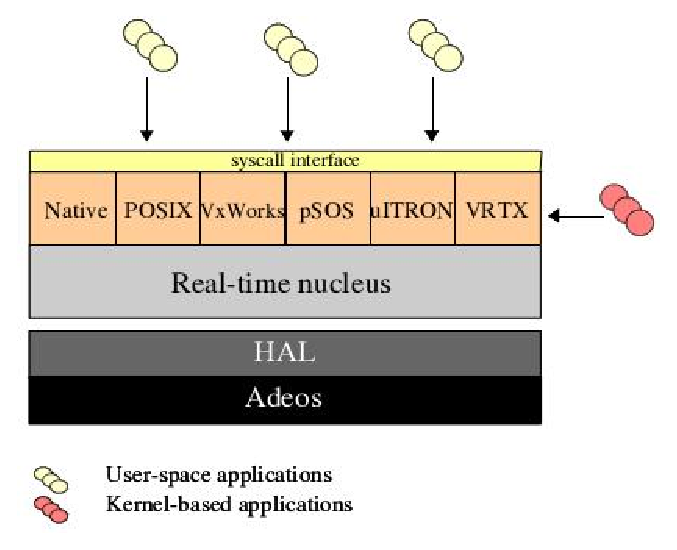
\includegraphics[scale=0.7]{xenomai_skins}
\caption{Skins para o Xenomai \cite{XENO_API06}}
\label{fig:xenomai_skins}
\end{figure}	
	
	O Xenomai utiliza como \textit{micro-kernel} o ADEOS \cite{ADEOS01}, uma camada de abstração do hardware que permite que vários sistemas operacionais compartilhem os recursos de hardware (Figura \ref{fig:xenomai_skins}). O ADEOS trabalha com o conceito de domínios, que são as entidades que coexistem na máquina, onde cada domínio não tem o conhecimento do outro mas todos se comunicam com o ADEOS \cite{ADEOS01}.

	As aplicações de tempo real que são desenvolvidas desde o início tendo como base o Xenomai, geralmente utilizam a API nativa \cite{XENO_API06} do Xenomai. Esta oferece vários serviços disponibilizados comumente nos RTOS \cite{VERGO01} \cite{KALINSKY03}. Os serviços são divididos em seis grandes categorias, sendo que as principais são: gerenciamento de tarefas, serviços de tempo, suporte à sincronização, além de comunicação e transferência de mensagens. Estes serviços podem ser chamados tanto no contexto do espaço do kernel como no contexto do espaço de usuário, permitindo que as aplicações possam executar nos dois contextos.
	
	O Xenomai permite que as tarefas de tempo real executem tanto no domínio do Xenomai (modo primário) como no domínio do Linux (modo secundário), de forma totalmente transparente para os desenvolvedores. Quando uma tarefa executando no domínio do Xenomai faz uma chamada de sistema ao Linux, esta migra para o domínio do Linux, passando a ser gerenciado por este. Quando a execução da chamada de sistema é finalizada, a tarefa volta para o domínio do Xenomai. Para que a previsibilidade possa continuar a ser provida mesmo quando uma tarefa está sob gerência do kernel do Linux, o Xenomai disponibiliza o escudo de interrupção (\textit{Interrupt shield}) \cite{XENO_API06}.
	
	Para que um sistema distribuído possa ter suas restrições de tempo atendidas, além de um kernel de tempo real, é necessário que o sistema de comunicação na rede também forneça garantias temporais. O projeto RTnet, descrito a seguir, visa atender tais requisitos.
	
\section{RTnet}

	O RTnet é um \textit{framework} para comunicação de tempo real rígido sobre Ethernet e outros meios de comunicação \cite{KWZB05}. Enquanto o Xenomai (apresentado anteriormente) se preocupa basicamente com o escalonamento das tarefas de tempo real (está relacionado com o processamento das mensagens), o RTnet foca a transferência das mensagens sobre uma rede Ethernet com restrições rígidas de tempo. Neste caso, podemos observar que o Xenomai e o RTnet se complementam na função de fornecer uma solução para a comunicação em rede que atenda às restrições rígidas de tempo.
	
	Basicamente o RTnet consiste em uma pilha de protocolos de rede capaz de prover comunicação de tempo real sobre Ethernet. Para garantir as restrições rígidas de tempo, o RTnet implementa os protocolos UDP/IP, ICMP e ARP retirando todas as possíveis causas de indeterminismo \cite{KWZB05}.
	
	Além da implementação dos protocolos de forma determinística, o RTnet provê um controle de acesso ao meio determinístico através de sua camada de acesso ao meio denominada RTmac. Com o RTmac, as aplicações de tempo real conseguem obter QoS a um custo baixo, visto que não dependem que um \textit{hardware} implemente a solução de QoS \cite{KWZB05}. Por padrão, a disciplina de acesso ao meio utilizada pelo RTnet para se comunicar na rede Ethernet é o TDMA (\textit{Time Division Multiple Access}). Esta disciplina segue a abordagem mestre-escravo, onde o nó mestre no segmento Ethernet é responsável por sincronizar os relógios dos nós escravos e por definir o momento em que estes podem enviar seus pacotes.
% !TEX encoding = UTF-8 Unicode
%\chapter{Especificação do QoSPM}
\xchapter{Especificação do QoSPM}{}
\label{cap:especificacao}
\acresetall

	Neste capítulo o QoSPM será especificado, sendo que ele está dividido em quatro seções: na seção 5.1 será descrita a arquitetura do QoSPM; na 5.2 a modelagem do QoSPM através da UML será abordada; na 5.3 será descrito o protocolo utilizado pelos componentes do QoSPM; e para finalizar, a seção 5.4 abordará os principais algoritmos utilizados pelo QoSPM.

\section{Arquitetura do QoSPM}

	A arquitetura do QoSP foi descrita no caítulo \ref{cap:qos_provider}. Agora nós iremos focar a arquitetura do QoSP \textit{Monitoring}. Como foi descrito anteriormente, uma rede com o QoS \textit{Provider} é formada por módulos do QoSP e por roteadores. Além destes elementos, um novo elemento foi adicionado para compor a arquitetura do QoS \textit{Provider}, mas especificadamente do QoSPM, sendo denominado QoSP \textit{Agent} (QoSPA). Para cada roteador existe um módulo do QoSPA, sendo que este tem a função de monitorar o roteador que está vinculado ao mesmo (Figura \ref{fig:arquitetura_qosp}).
	
\begin{figure}
\centering
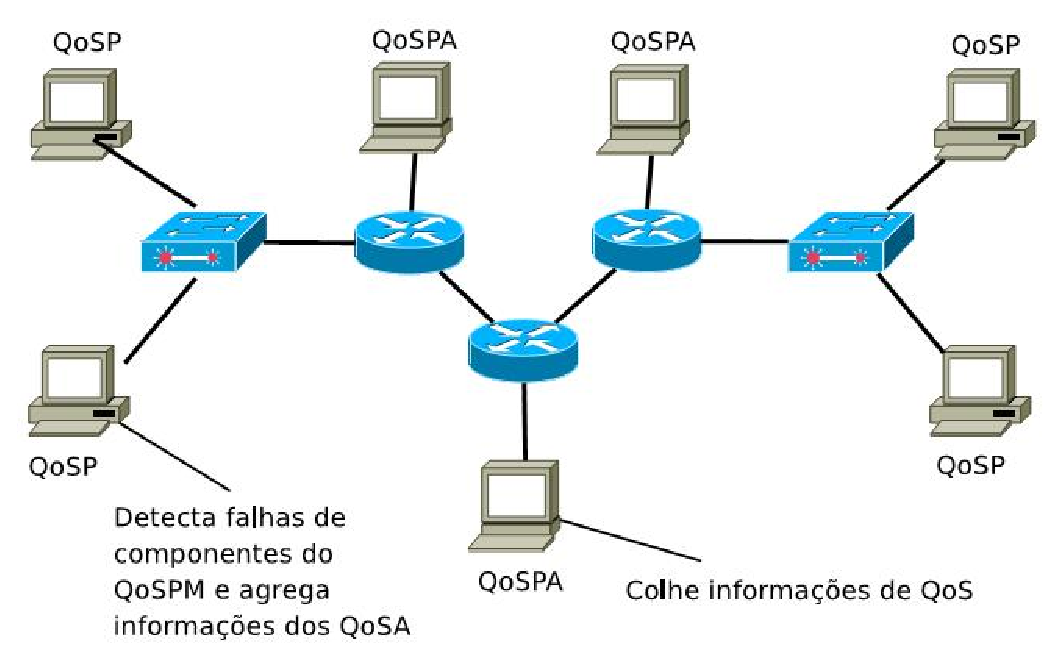
\includegraphics[scale=0.7]{arquitetura_qospm}
\caption{Arquitetura do QoSPM}
\label{fig:arquitetura_qosp}
\end{figure}

\subsection{O QoSP}
	Os módulos do QoSP executam nos \textit{hosts}, sendo que estes \textit{hosts} são aqueles onde se localizam os componentes que caracterizam o modelo HA, assim como os processos distribuídos que executam sobre o modelo HA. Além dos módulos do QoSP trocarem mensagens entre si (como mensagens de requisição remota de verificação de canal), um determinado QoSP comunica-se com vários módulos do QoSPA para colher informações sobre a QoS que está sendo provida para um determinado canal (mas especificadamente para uma determinada classe de serviço da arquitetura Diffserv), cujos roteadores estão sendo monitorados pelos módulos do QoSPA com os quais a comunicação foi estabelecida. Depois de agregada as informações, a QoS do canal pode ser então descoberta. O QoSP também se comunica com o QoSPA para informar sobre seu interesse em receber informações relativas à degradação da QoS no roteador monitorado pelo QoSPA, com o intuito de antecipar o \textit{feedback} provido pelo mecanismo de monitoramento aos processos aplicativos. Sendo assim, a política de notificação de eventos é adotada (ver \ref{cap:qos}).
	
	A arquitetura utilizada pelo QoSP segue a abordagem distribuída adotada pelo modelo de monitoramento descrito no capítulo \ref{cap:qos}. Os componentes \textit{Monitoring Application} e \textit{QoS Monitoring} do modelo de monitoramento fazem parte do QoSP. Além das funções descritas anteriormente, o QoSP é responsável pela detecção de falhas dos elementos que são importantes para o funcionamento do QoSPM (roteadores, módulos do QoSP e módulos do QoSPA).
	
\subsection{O QoSPA}
	Cada módulo do QoSPA está vinculado a um roteador específico e sua função é colher informações sobre QoS no roteador vinculado ao mesmo. O QoSPA executa em um \textit{host} conectado diretamente ao roteador, seguindo um dos princípios de sistemas de monitoramento. Caso o QoSPA não possa executar em \textit{host} específico, o mesmo poderá executar em um \textit{host} onde se localiza um módulo do QoSP. O QoSPA colhe periodicamente informações de QoS, pré-processa e sumariza estas informações que serão utilizadas pelos módulos do QoSP. Neste contexto, o QoSPA funciona como um agente para o QoSP. O componente \textit{Monitor} do modelo de monitoramento faz parte do QoSPA. Seguindo os princípios de sistemas de monitoramento, o QoSPA executa distribuído (um para cada roteador), além das informações colhidas pelos mesmos serem no nível do agregado (no nível das classes do \textit{Diffserv}).
	
	O protocolo utilizado pelo QoSPA para colher informações de QoS é o SNMP. Uma das vantagens de se utilizar o SNMP é que dependendo da granularidade proporcionada pela MIB utilizada para obter informações de QoS, quanto mais específicas forem as variáveis definidas na MIB, menos mensagens serão trocadas entre o QoSPA e o roteador para se obter uma informação mais robusta. O QoSPA utiliza o SNMP para verificar se a QoS que havia sido previamente negociada para um canal continua sendo provida, verificando se a classe Serviço Expresso configurada no roteador continua provendo seus serviços da maneira esperada. Caso seja percebido que ocorreu degradação, todos os módulos do QoSP interessados em receber tal informação serão notificados.
	
\section{Modelagem do QoSPM}
	A especificação do QoSPM foi feita através da modelagem do sistema utilizando a abordagem orientada à objetos, sendo que tal modelagem foi feita utilizando-se a UML \cite{UML99}. Com a modelagem, além de ser possível especificar a estrutura e comportamento do sistema, as decisões tomadas são documentadas \cite{UML99}.
	
	Baseado na arquitetura descrita na seção anterior e na funcionalidade provida pelo mecanismo de monitoramento, a estrutura do QoSPM foi especificada através de diagramas de classe. Foram desenvolvidos diagramas de classe para modelar tanto o QoSP como o QoSPA.
	
\subsection{QoSP}
	Por ser o módulo principal, o QoSP envolveu tanto a modelagem do domínio como a modelagem da aplicação. O domínio representa o vocabulário inerente ao mecanismo de monitoramento do QoS \textit{Provider}. As informações do vocubulário que necessitam serem armazenadas são relativas aos canais de comunicação. O modelo de classes do domínio (Figura \ref{fig:diagrama_classe_dominio}) é formado pelas seguintes entidades:
	
\begin{figure}
\centering
%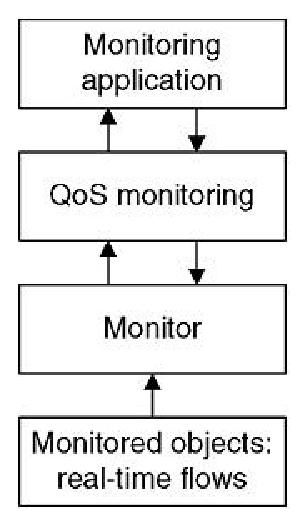
\includegraphics[width=0.3\textwidth]{modelo}
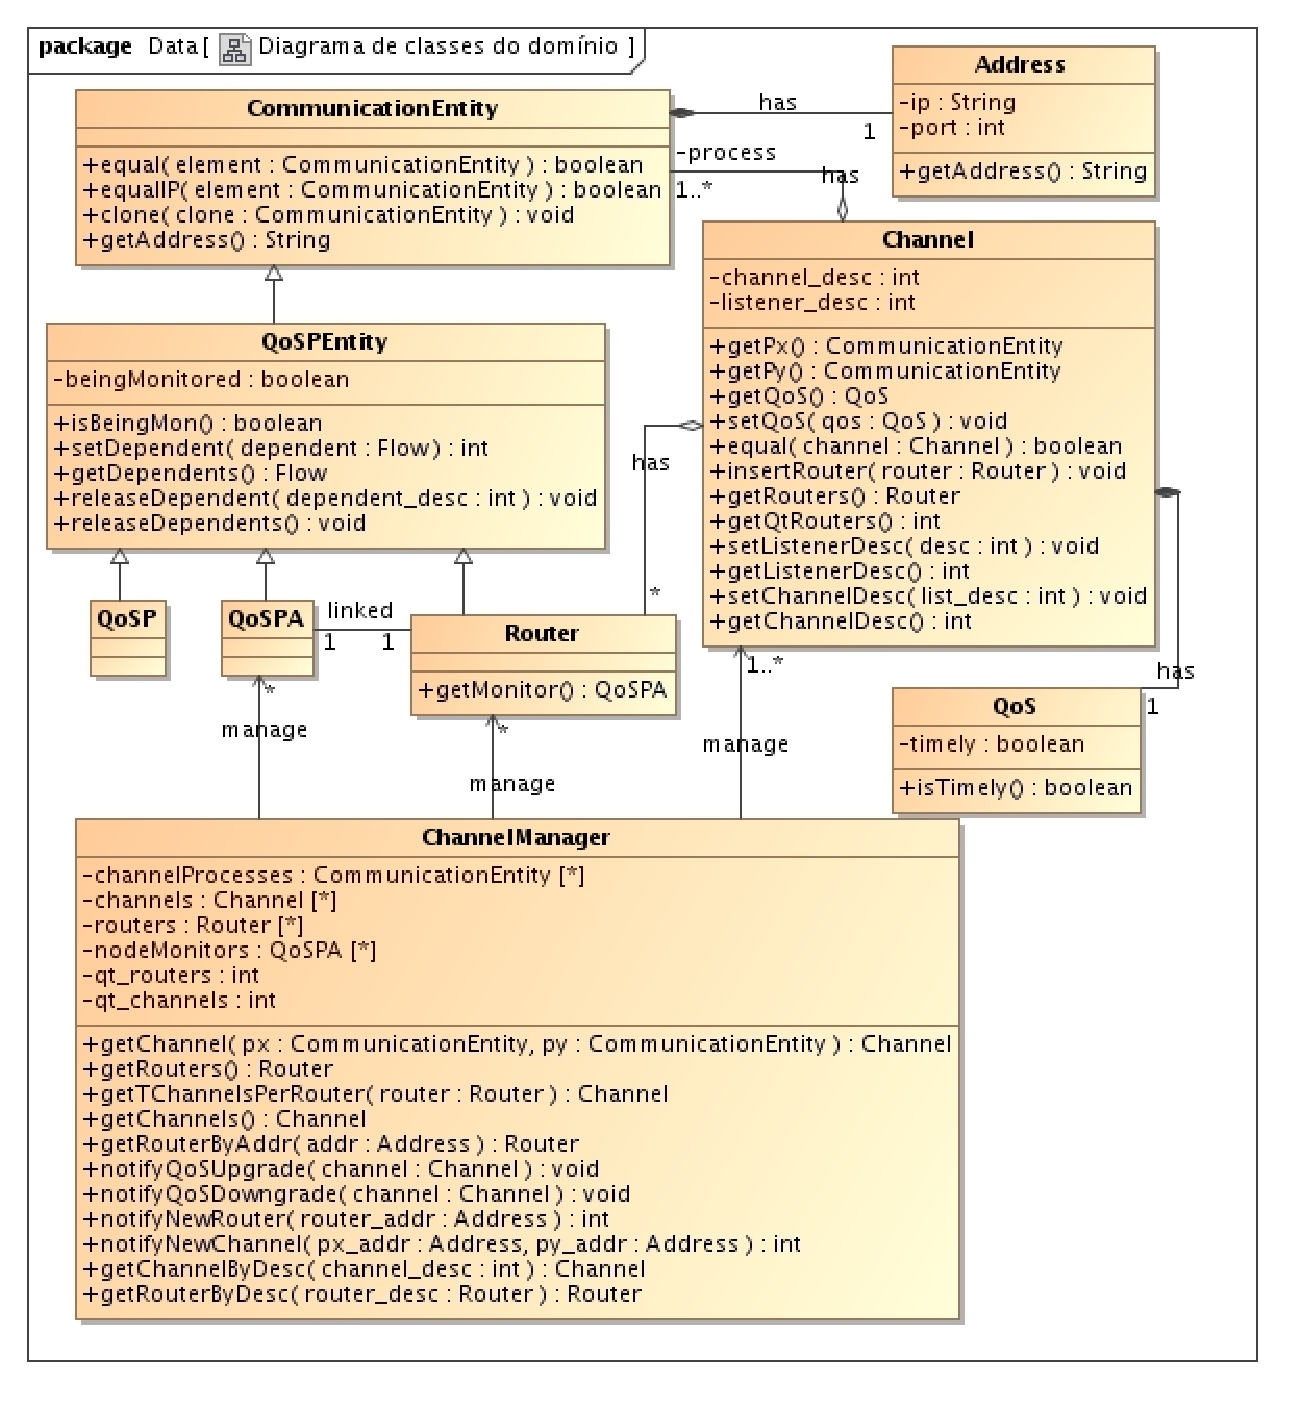
\includegraphics[scale=0.7]{diagrama_dominio}
\caption{Diagrama de classes do Domínio}
\label{fig:diagrama_classe_dominio}
\end{figure}
	
\begin{itemize}
\item \textbf{CommunicationEntity}: Representa qualquer entidade com a qual se possa estabelecer uma comunicação na rede. Essa entidade pode ser tanto um componente de \textit{software} como um componente de \textit{hardware}. Para que essa comunicação seja possível, essa entidade necessita ser localizada através de um endereço IP.

\item \textbf{Address}: Representa um endereço IP de uma \textit{CommunicationEntity}.

\item \textbf{QoSPEntity}: Limita o escopo do que uma \textit{CommunicationEntity} pode ser, mas especificadamente, especifica as entidades que compõem o QoSPM e que, possivelmente, necessitarão ser monitoradas.

\item \textbf{QoSP}: Representa um módulo do QoSP.

\item \textbf{QoSPA}: Representa um módulo do QoSPA.

\item \textbf{Router}: Representa um roteador.

\item \textbf{Channel}: Representa um canal lógico, formado por dois processos e por roteadores.

\item \textbf{QoS}: Representa a QoS de um \textit{Channel}. No contexto do QoSPM, a QoS de um canal só pode ser \textit{TIMELY} ou \textit{UNTIMELY}.

\item \textbf{ChannelManager}: Gerencia o principal recurso do QoS \textit{Provider}, os canais, além dos componentes do QoSPM cujas informações necessitam serem recuperadas pelas classes do modelo de aplicação. É importante salientar que \textit{ChannelManager} gerencia apenas os recursos que, de certa forma, estão relacionados aos canais de comunicação cujos processos localizam-se em seu \textit{host}.	
\end{itemize}
	
	O modelo de aplicação define a aplicação (mecanismo de monitoramento) propriamente dita, e não os objetos (definidos no modelo de domínio) sobre os quais a aplicação atua \cite{BLAHUM06}. A maioria das classes deste modelo são orientadas a computação, diferentemente do modelo de domínio. O modelo de classes da aplicação (Figura \ref{fig:diagrama_classe_qosp}) é formado pelas seguintes entidades:
	
\begin{figure}
\centering
%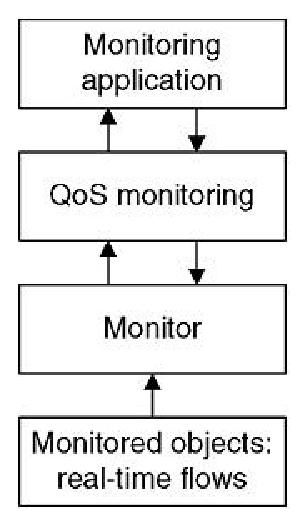
\includegraphics[width=0.3\textwidth]{modelo}
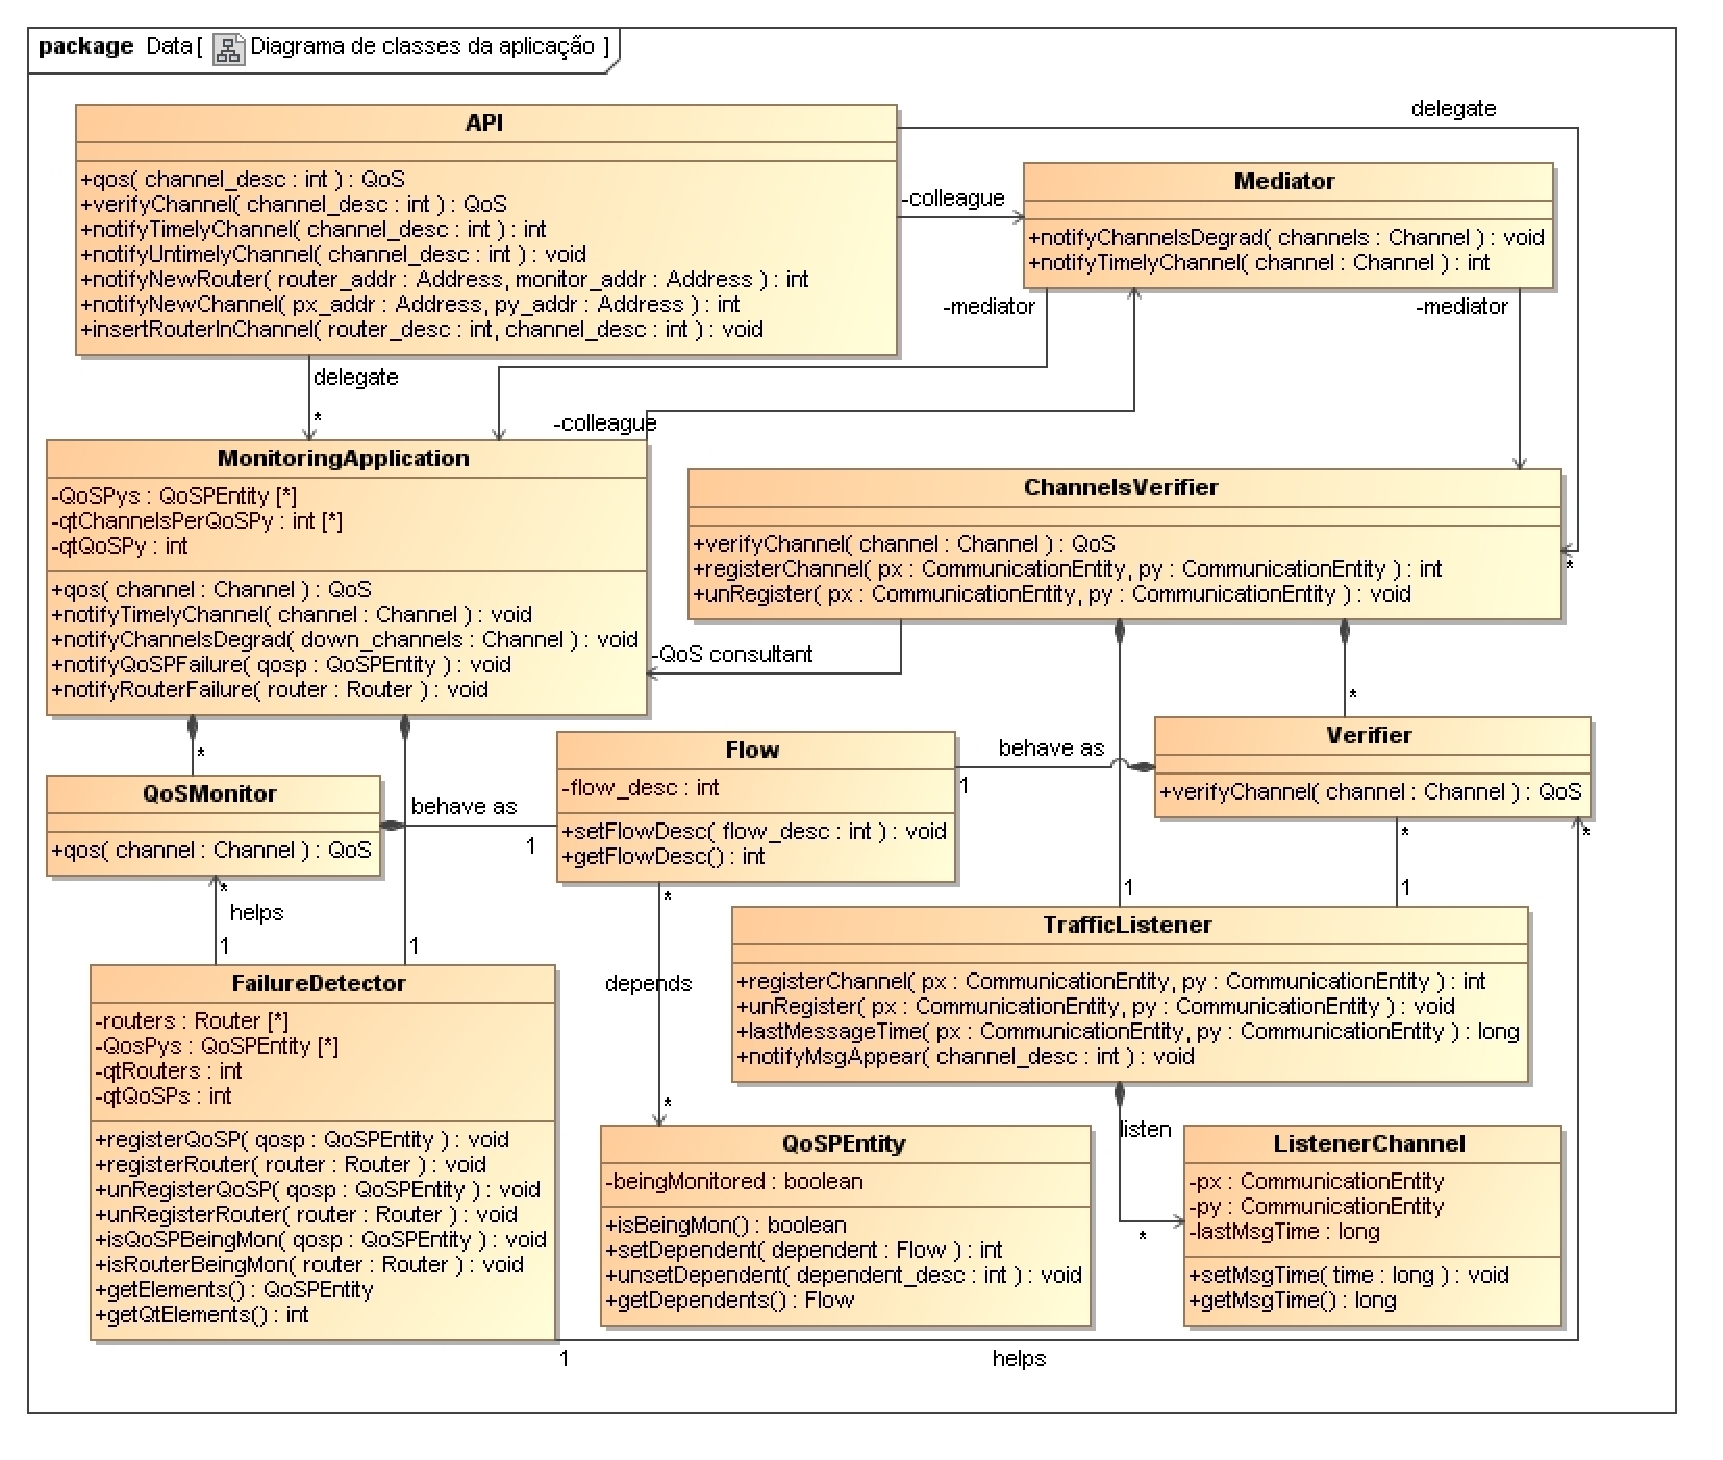
\includegraphics[scale=0.65]{diagrama_aplicacao}
\caption{Diagrama de classes do QoSP}
\label{fig:diagrama_classe_qosp}
\end{figure}	
	
\begin{itemize}
\item \textbf{API}: Representa a interface do QoSPM. Como foi descrito no capítulo \ref{cap:qos_provider}, tanto os processos aplicativos como o módulo de negociação necessitam interagir com o QoSPM. Ambos enxergam o QoSPM através desta classe.

\item \textbf{Mediator}: Encapsula como os objetos das classes \textit{API}, \textit{MonitoringApplication} e \textit{ChannelVerifier} interagem quando há altereção de QoS de um canal. Esta classe modela o principal participante do padrão de projeto \textit{Mediator} \cite{GAHEJOVLI97}.

\item \textbf{MonitoringApplication}: É responsável por delegar cada monitoração de QoS para um \textit{QoSMonitor}. Além disso ela também é responsável por verificar quando um determinado módulo do QoSP não necessita mais ser monitorado pelo \textit{FailureDetector}, visto que não existem mais canais passando pelo \textit{host} do mesmo.

\item \textbf{QoSMonitor}: É responsável por monitorar a QoS de um canal, quando tal monitoramento é requisitado.

\item \textbf{FailureDetector}: Responsável por monitorar periodicamente objetos \textit{QoSPEntity} à procura de falhas. Caso falhas sejam detectadas, objetos \textit{QoSMonitor} assim como objetos \textit{Verifier} podem usufruir de tal informação, visto que, possivelmente, respostas das mensagens enviadas pelos mesmos não chegarão. É importante salientar que \textit{FailureDetector} é a única classe que necessita estabelecer \textit{timeouts} para a recepção de respostas às suas mensagens enviadas. Tanto \textit{QoSMonitor} como \textit{Verifier} não necessitam estabelecer \textit{timeouts} para a execução de suas funções, visto que eles contam com informações providas por \textit{FailureDetector} sobre falhas em componentes que impediriam suas respostas de chegarem.

\item \textbf{ChannelVerifier}: É responsável por delegar cada verificação de canal para um \textit{Verifier}. Além disso ela também é responsável por informar \textit{TrafficListener} quando canais de comunicação devem ou não ser escutados.

\item \textbf{Verifier}: É responsável por realizar a verificação de canal (descrita no capítulo \ref{cap:qos_provider}), quando tal verificação é requisitada.

\item \textbf{TrafficListener}: Responsável por escutar os canais de comunicação e armazenar informações sobre o momento em que houve tráfego nestes canais.

\item \textbf{ListenerChannel}: Representa um canal de comunicação que está sendo escutado por \textit{TrafficListener}.

\item \textbf{Flow}: Modela o comportamento de um fluxo de execução. Tanto \textit{QoSMonitor} como \textit{Verifier} se comportam como um fluxo de execução, visto que tanto a função de monitoração de QoS como a função de verificação de canal podem ter mais de uma requisição sendo realizada ao mesmo tempo.

\end{itemize}

\subsection{QoSPA}

	O módulo do QoSPA tem uma funcionalidade bem mais restrita se comparado ao módulo do QoSP. O diagrama de classes (Figura \ref{fig:diagrama_classe_qospa}) do mesmo é bem simples, sendo formado pelas seguintes classes:
	
\begin{figure}
\centering
%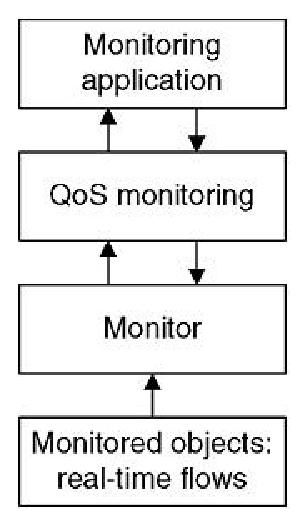
\includegraphics[width=0.3\textwidth]{modelo}
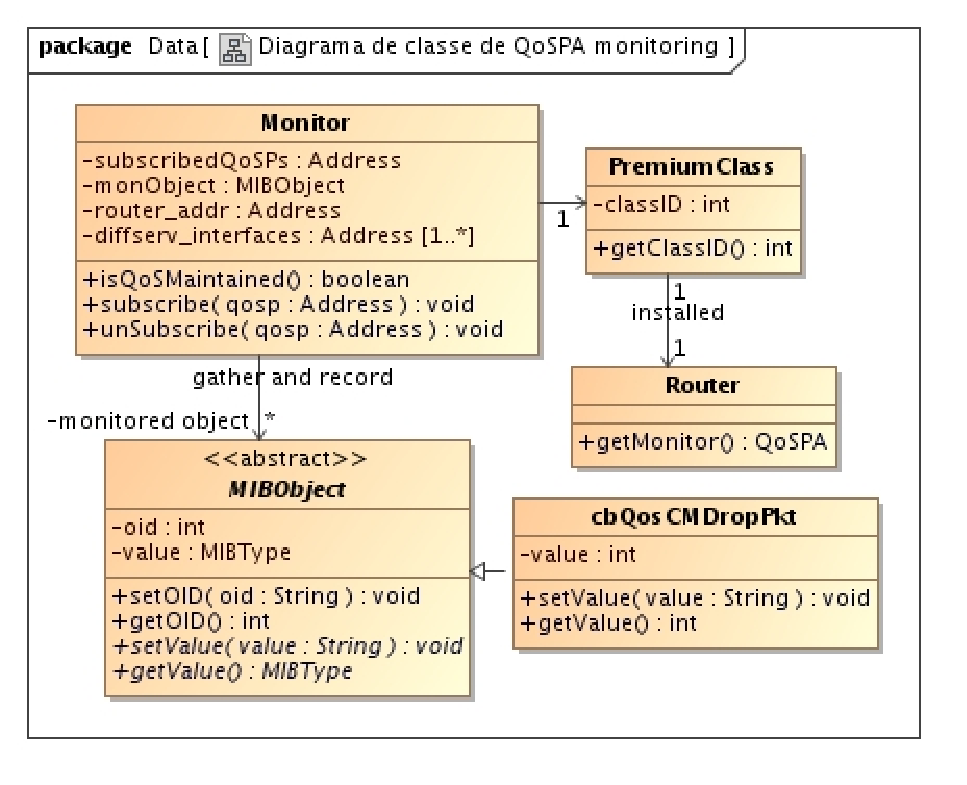
\includegraphics[scale=0.7]{diagrama_qospa}
\caption{Diagrama de classes do QoSPA}
\label{fig:diagrama_classe_qospa}
\end{figure}

\begin{itemize}
\item \textbf{Monitor}: É responsável por colher informações, provenientes do roteador vinculado ao módulo QoSPA do qual faz parte, relativas à classe do serviço Expresso. Essas informações serão utilizadas para verificar se a QoS anteriormente negociada continua sendo provida. Essas informações colhidas correspondem aos \textit{MIBObject}s.

\item \textbf{MIBObject}: Representa um objeto MIB (explicado na seção que descreve o SNMP no capítulo \ref{cap:qos}) colhido por \textit{Monitor}. Cada \textit{MIBObject} corresponde a um \textit{Monitored object} do modelo conceitual de monitoramento (descrito no capítulo \ref{cap:qos}). Essa classe é abstrata pois o tipo do valor de cada objeto MIB pode variar. O objeto MIB capturado deve implementar os métodos abstratos desta classe.

\item \textbf{PremiumClass}: Representa a classe de serviço expresso configurada em um roteador.
\end{itemize}

\section{Protocolo utilizado pelo QoSPM}
	Como foi descrito nas seções anteriores, o QoSPM é composto por módulos do QoSP e do QoSPA que trocam mensagens entre si e com os roteadores. Para descrever tais mensagens, foi definido um protocolo de comunicação. A seguir serão descritas as mensagens que fazem parte do protocolo, sendo que para cada mensagem serão descritos o componente que enviou tal mensagem, o componente receptor, em qual contexto assim como a semântica da mensagem enviada, os campos que compõem a mensagem (toda mensagem possui um campo que identifique o tipo da mensagem, sendo assim este não será citado) e, se houver a necessidade, a ordem de precedência com relação a outras mensagens. A palavra \textit{QoSP} será utilizada de forma intercambiável com a expressão \textit{módulo do QoSP} assim como a palavra \textit{QoSPA} será utilizada de forma intercambiável com a expressão \textit{módulo do QoSPA}, ambos os módulos descritos na seção inicial deste capítulo.
	
\begin{itemize}
\item \textbf{Monitoring Request}: Esta mensagem é enviada por um QoSP para um QoSPA quando uma requisição de monitoramento (função \textit{QoS} descrita no capítulo \ref{cap:qos_provider}) de QoS é executada. Requisita ao QoSPA que verifique junto ao roteador vinculado ao mesmo se a classe Serviço Expresso configurada neste roteador continua provendo seus serviços da maneira esperada. Tal mensagem possui um campo que identifica uma requisição de monitoramento específica, visto que várias requisições de monitoramento podem ser feitas ao mesmo tempo. Além disso, ela possui um campo que identifica unicamente uma mensagem deste tipo, visando descartar mensagens antigas.

\item \textbf{Monitoring Reply}: Esta mensagem é enviada por um QoSPA para um QoSP em resposta à mensagem \textit{Monitoring Request} previamente enviada. Depois que QoSPA verifica junto ao roteador vinculado ao mesmo se a classe Serviço Expresso configurada neste roteador continua provendo seus serviços da maneira esperada, ele manda a resposta ao QoSP. Tal mensagem possui um campo que informa se a QoS está mantida, além de dois outros campos cujos valores e tipos são os mesmos da mensagem \textit{Monitoring Request} recebida.

\item \textbf{Monitoring Reply Ack.}: Esta mensagem é enviada por um QoSP para um QoSPA em resposta à mensagem \textit{Monitoring Reply} previamente recebida, sendo que na mensagem \textit{Monitoring Reply} consta que houve degradação da QoS. Depois que o QoSP recebeu do QoSPA a resposta do monitoramento e descobriu que houve degradação, ele deve enviar uma mensagem de reconhecimento. Isto é importante pois como ocorreu degradação, a resposta do monitoramento pode não ter sido entregue ao QoSP. Tal mensagem possui dois campos cujos valores e tipos são os mesmos dos dois últimos campos de \textit{Monitoring Reply}.

\item \textbf{Verification Request}: Esta mensagem é enviada por um QoSP para outro QoSP quando uma requisição de verificação de canal (função \textit{Verify Channel} descrita no capítulo \ref{cap:qos_provider}) é executada, sendo que o canal em questão não é gerenciado pelo QoSP local (uma requisição remota deve ser executada). Tal mensagem requisita ao QoSP remoto que faça uma verificação local do canal em questão. Tal mensagem possui um campo que identifica os dois processos (através dos endereços IP) que fazem parte do canal a ser verificado. Além disso, esta mensagem possui dois outros campos semelhantes aos campos  de \textit{Monitoring Request}.

\item \textbf{Verification Reply}: Esta mensagem é enviada por um QoSP para outro QoSP em resposta à mensagem \textit{Verification Request} previamente enviada. Depois que o QoSP verifica localmente um canal (através da execução da função \textit{Verify Channel}), ele manda a resposta ao QoSP que havia solicitado a verificação remota. Tal mensagem possui um campo com o resultado da verificação local, além de dois outros campos cujos valores e tipos são os mesmos dos dois últimos campos de \textit{Verification Request}.

\item \textbf{Subscribe}: Esta mensagem é enviada por um QoSP para um QoSPA quando um canal teve sua QoS alterada para \textit{TIMELY}, sendo que o QoSPA em questão ainda não havia recebido tal mensagem anteriormente. O QoSP envia tal mensagem ao QoSPA para informar que está interessado em receber informações sobre degradação da QoS provida pelo roteador no qual o QoSPA está vinculado. O intuito desta mensagem é de antecipar a informação sobre degradação da QoS, consequentemente antecipar o \textit{feedback} provido pelo QoSPM. Esta mensagem não possui nenhum campo adicional.

\item \textbf{Unsubscribe}: Esta mensagem é enviada por um QoSP para um QoSPA quando a QoS de todos os canais, que passam pelo roteador vinculado ao QoSPA em questão e que são gerenciados pelo QoSP, foi rebaixada para \textit{UNTIMELY}. O QoSP envia tal mensagem ao QoSPA para informar que não está mais interessado em receber informações sobre degradação da QoS provida pelo roteador no qual o QoSPA está vinculado. Esta mensagem não possui nenhum campo adicional.

\item \textbf{Notify Degradation}: Esta mensagem é enviada por um QoSPA para um(ns) QoSP(s) quando, depois que informações de QoS são colhidas e pré-processadas, percebe-se que houve degradação da QoS provida pelo roteador. Tal mensagem é enviada para todos os QoSPs que estão interessados em receber informação de degradação de QoS no roteador vinculado ao QoSPA em questão. Esta mensagem não possui nenhum campo adicional.

\item \textbf{Are you alive}: Esta mensagem é enviada por um QoSP (mas especificadamente pelo detector de falhas do QoSP) para um QoSP/QoSPA/roteador periodicamente. Tal mensagem tem por objetivo verificar se um determinado componente do QoSPM falhou. Esta mensagem equivale a um \textit{Echo Request} do protocolo ICMP. Possui um campo que identifica unicamente uma mensagem deste tipo, além de um campo que identifica o elemento (QoSP ou QoSPA ou roteador) para o qual está sendo enviada a mensagem. Este campo é necessário para que o detector de falhas possa saber quais os elementos que responderam a esta mensagem dentro do limite temporal.

\item \textbf{Explicit ping}: Esta mensagem é semelhante à \textit{Are you alive}, mas ela é enviada para um QoSP quando uma requisição de monitoramento de QoS é executada. O QoSP para o qual a mensagem é enviada localiza-se no mesmo \textit{host} de $p_{y}$, sendo $p_{y}$ o processo remoto do canal cuja monitoração foi solicitada. Esta mensagem, em complemento às mensagens \textit{Monitoring Request} enviadas, são necessárias para a execução do monitoramento de QoS. Esta mensagem não possui um campo que identifica o elemento para o qual a mensagem foi enviada, mas possui um campo que identifa uma requisição de monitoramento específica. 

\item \textbf{I am alive}: Esta mensagem é enviada por um QoSP/QoSPA/roteador para um QoSP em resposta à mensagem \textit{Are you alive} (ou \textit{Explicit ping}) previamente recebida. Ela equivale a um \textit{Echo Reply} do protocolo ICMP. Tal mensagem possui dois campos cujos valores e tipos são os mesmos da mensagem \textit{Are you alive} (ou \textit{Explicit ping}) recebida.
\end{itemize}

	Além das mensagens descritas acima, o QoSPM utiliza mensagens SNMP (estas não fazem parte do protocolo definido visto que o SNMP já é um protocolo padronizado) na sua comunicação. As mensagens SNMP são trocadas entre o QoSPA e o roteador vinculado ao mesmo, e tem por objetivo colher informações de QoS. As seguintes mensagens foram utilizadas:
	
\begin{itemize}
\item \textbf{Get Request}: Enviada por um QoSPA para o roteador vinculado ao mesmo quando o QoSPA deseja verificar se a QoS continua sendo mantida. Esta mensagem é utilizada para capturar o valor de uma ou mais variáveis MIB (descritas no capítulo \ref{cap:qos}).

\item \textbf{Get Response}: Enviada por um roteador para o QoSPA no qual está vinculado em resposta à mensagem \textit{Get Request} previamente recebida. Ela contém os valores das variáveis MIB requisitados.
\end{itemize}	

\section{Algoritmos do QoSPM}

	Para completar o desenvolvimento do QoSPM, os algoritmos que o compõe foram especificados. Para cada algoritmo será descrita sua funcionalidade, assim como o contexto em que o mesmo executa. As mensagens citadas na descrição dos algoritmos são as mesmas descritas na seção anterior. Assim como na seção anterior, a palavra \textit{QoSP} será utilizada de forma intercambiável com a expressão \textit{módulo do QoSP} assim como a palavra \textit{QoSPA} será utilizada de forma intercambiável com a expressão \textit{módulo do QoSPA}.

%macros definidas por mim
\SetKwFor{AtEvery}{At every}{do}{end}
\SetKw{Task}{Task}
\SetKw{Execute}{execute}
\SetKw{Wait}{wait for}
\SetKwFor{When}{when}{do}{end}
%fim

\begin{itemize}
\item \textbf{Failure Detector} (Algoritmo 1): Algoritmo composto por duas tarefas que executam em paralelo no contexto do \textit{Failure Detector} do QoSPM. Tais tarefas são responsáveis por detectar a falha dos componentes do QoSPM, mas especificadamente QoSP, QoSPA e roteadores. É importante ressaltar que cada QoSP monitora apenas os componentes que estão relacionados com os canais gerenciados pelo mesmo. A tarefa \textit{detectFailure} é responsável por enviar periodicamente mensagens \textit{"Are you alive ?"} para os componentes de interesse do QoSP. A periodicidade do monitoramento é definido através do parâmetro \textit{FD monitoring interval}. O vetor \textit{elements} armazena os componentes que devem ser monitorados. A função \textit{getElements()} retorna os elementos que devem ser monitorados ordenados pelo tempo de transferência de mensagens entre o QoSP local e o componente em questão, sendo que este tempo é calculado pela função \textit{Delay}. A variável \textit{ExpectedMsg} identifica o elemento cuja mensagem \textit{"I am alive"} possivelmente será a próxima a ser recebida. Esta variável é compartilhada pelas duas tarefas. O vetor \textit{ReplyStatus} guarda a informação dos elementos cujas mensagens \textit{"I am alive"} já chegaram. Este vetor também é compartilhado pelas duas tarefas. A função \textit{CT()} retorna a hora local. A declaração \textit{Set EventWait(EVENT, timeout)} serve para indicar que a ocorrência de um evento será aguardada ou a ocorrência de um \textit{timeout}, o que vier primeiro. Basicamente, o algoritmo funciona da seguinte maneira: baseado nas mensagens \textit{"I am alive"} que ainda não chegaram, a função \textit{EventWait} configura o \textit{timeout} para o elemento cuja mensagem \textit{"I am alive"} é a próxima esperada. Quando uma determinada mensagem não chegou no tempo esperado, é notificada a falha do componente correspondente. Uma vantagem deste algoritmo é que com apenas uma única \textit{thread} de execução é possível monitorar todos os elementos concorrentemente, sendo que o tempo máximo para executar uma rodada deste algoritmo corresponde ao \textit{delay} calculado para o último elemento do vetor \textit{elements}.

	A tarefa \textit{fdListener} é responsável por ficar escutando o canal do \textit{Failure Detector} e atualizando \textit{ReplyStatus} com as informações dos elementos cujas mensagens \textit{"I am alive"} já chegaram. Além do mais, ela é responsável por sinalizar a chegada da mensagem esperada.
	
\SetAlgoSkip{0em}
\SetAlgoInsideSkip{0em}
\SetAlCapSkip{0em}
\SetVlineSkip{0em}
\setlength{\algomargin}{0em}
%\Setnlskip{0em}
\SetAlFnt{\small}
%\SetDataSty{}
%\SetInd{0em}{0em}
%\SetAlTitleFnt{textit}
%\SetAlFont{\small\em}	
%\begin{algorithm}[H]
\begin{algorithm}[H]
%AlFont{\small\em}
%\dontprintsemicolon
%\SetVline
%\KwData{elements}
%\KwData{ExpectedMsg}
%\KwData{ReplyStatus}
\Task{detectFailure}\;
\Begin{
\AtEvery{FD monitoring interval}{
	%$elements \leftarrow$ FD.getElements()\;
	$elements \leftarrow getElements()$\;
	$ExpectedMsg \leftarrow 1$\;
	\ForEach{$element \in elements$}{
	$ReplyStatus[element] \leftarrow NotReceived$\;
	$AliveMsg.id \leftarrow element$\;
	$MsgSentTime[element] \leftarrow CT()$\;
	send $"AliveMsg"$ message to $element$\;
	}
	
	\textbf{Set} EventWait($ExpectedMsgReceived$, Delay(localQoSP, $elements[1]$))\;
	\ForEach{$element \in elements$}{
		\If{$ReplyStatus[element] = NotReceived$}{
			\If{$element = ExpectedMsg$}{
				\If{$element.type = QoSP$}{
					%FD.notifyQoSPFailure($element$)\;
					$notifyQoSPFailure(element)$\;
				}
				\ElseIf{$element.type = QoSPA$}{
					$notifyQoSPAFailure(element)$\;
				}
				\Else{
					%FD.notifyRouterFailure($element$)\;
					$notifyRouterFailure(element)$\;
				}
				\lIf{element is the last}{$continue$\;}
				$ExpectedMsg \leftarrow ExpectedMsg + 1$\;				
				%\textbf{Set} EventWait($ExpectedMsgReceived$, $MsgSentTime[ExpectedMsg] + Delay(localQoSP, \; elements[ExpectedMsg] - CT()$))\;
			}
			\Else{
				$ExpectedMsg \leftarrow element$\;
				%\textbf{Set} EventWait($ExpectedMsgReceived$, $MsgSentTime[ExpectedMsg] + Delay(localQoSP, elements[ExpectedMsg] - CT()$))\;
			}
			\textbf{Set} EventWait($ExpectedMsgReceived$, $MsgSentTime[ExpectedMsg] + Delay(localQoSP, elements[ExpectedMsg]) - CT()$)\;
		}
	}
}
}

\Task{fdListener}\;
\Begin{
	%\When{AliveMsgReply is received}{
	\textbf{wait for}(receive message $"AliveMsgReply"$)\;
		$ReplyStatus[AliveMsgReply.id] \leftarrow Received$\;
		\If{$ExpectedMsg = AliveMsgReply.id$}{
			SignalEvent($ExpectedMsgReceived$)\;
		}
	%}
}
\caption{Failure Detector}
\end{algorithm}	

\item \textbf{QoS} (Algoritmo 2): Responsável por verificar a QoS que está sendo provida ao canal de comunicação $c_{x/y}$ (equivale à função $QoS(p_{x}, p_{y})$ descrita no capítulo \ref{cap:qos_provider}). Esse algoritmo executa a tarefa \textit{checkQoSP} em paralelo com o resto do algoritmo. A tarefa \textit{checkQoSP} é responsável por verificar se um QoSP está vivo, através do envio da mensagem $"ExplicitPing"$. Caso a resposta não chegue dentro do \textit{timeout}, o resultado da verificação será \textit{UNTIMELY}. Para verificar a QoS do canal $c_{x/y}$, o algoritmo verifica se $QoSP_{y}$ está vivo além de enviar mensagens $"MonitoringRequest"$ para os QoSPA dos roteadores pertencentes ao canal $c_{x/y}$. Se todas as respostas dos QoSPA chegarem, informando que a QoS está mantida, o resultado da verificação é \textit{TIMELY}, caso contrário será \textit{UNTIMELY}. Observe que exceto pela tarefa \textit{checkQoSP}, o algoritmo não estabelece \textit{timeout} para o recebimento das mensagens. Visto que os canais do QoS Provider usufruem dos serviços isócronos, caso as mensagens não cheguem, foi decorrente da falha de um componente do QoSPM, cuja falha será notificada pelo \textit{Failure Detector}.

\begin{algorithm}[H]
	\Task{checkQoSP($QoSP_{y}$)}\;
	\Begin{
		$AliveMsg.id \leftarrow ExplicitPing$\;
		send $"AliveMsg"$ message to $QoSP_{y}$\;
		$timeout \leftarrow CT() + Delay(localQoSP, QoSP_{y})$\;
		%\When{$CT\left(\right) > timeout \vee AliveMsgReply \; is \; received$}{
		%\textbf{wait for}((receive message $AliveMsgReply$ from $QoSP_{y}$) \vee \; ($CT() > timeout$))\;
		\textbf{wait for}($(receive \; message \; AliveMsgReply \; from \; QoSP_{y}) \vee (CT() > timeout)$)\;
		\If{$CT\left(\right) > timeout$}{
			\Return{UNTIMELY}\;
		}
		%}
	}
	
	\Execute{checkQoSP($QoSP_{y}$)}\;
	\ForEach{$router \in channels[c_{x/y}]$}{
		send $"MonitoringRequest"$ message to QoSPA(router)\;
	}
	%\textbf{wait for}(((receive message $MonitoringReply(maintained)$ from QoSPA(router)) \vee \; (router \; has \; failed)) \; $\forall router \in channels[c_{x/y}]$)\;
	\textbf{wait for}($((receive \; message \; MonitoringReply(maintained) \; from \; QoSPA(router)) \vee  (router \vee QoSPA(router) \; has \; failed)) \; \forall router \in channels[c_{x/y}]$)\;
	\If{received every message MonitoringReply(maintained) $\wedge$ \; ($\forall message \; MonitoringReply(maintained), \; maintained = True$)}{
		\Return{TIMELY}\;
	}
	\Else{
		\Return{UNTIMELY}\;
	}
\caption{QoS($p_{x}, p_{y}$)}
\end{algorithm}

\item \textbf{VerifyChannel} (Algoritmo 3): Equivale à função $VerifyChannel(c_{x/y})$ descrita no capítulo três. Caso o canal $c_{x/y}$ não seja gerenciado pelo QoSP local, uma requisição remota será executada atráves do envio da mensagem $"VerificationRequest"$. O resultado da verificação remota será o resultado da função. Assim como no algoritmo $QoS(p_{x}, p_{y})$, não utiliza-se \textit{timeout}. Caso o canal seja gerenciado localmente, o resultado da função será encontrado através da execução da função \textit{QoS}, seguido de uma verificação de tráfego no canal, se necessário. O resultado da função \textit{VerifyChannel} será \textit{TIMELY} se o resultado da execução da função \textit{QoS} for \textit{TIMELY} e logo em seguida for percebido que houve tráfego no canal $c_{x/y}$ durante um certo intervalo de tempo (estabelecido pelo modelo HA). Caso contrário o resultado da função será \textit{UNTIMELY}.

\begin{algorithm}[H]
	\If{$c_{x/y} \notin channels$}{
		send $"VerificationRequest(c_{x/y})"$ message to $QoSP_{x}$\;
		\textbf{wait for}((received message $VerificationReply(c_{x/y},qos)$ from $QoSP_{x}$) $\vee$ \; ($QoSP_{x}$ has failed))\;
		\If{$received \; message \; VerificationReply(c_{x/y}, \; qos) \wedge qos = TIMELY$}{
			\Return{TIMELY}\;
		}
		\Else{
			\Return{UNTIMELY}\;
		}
	}
	\Else{
		$qos \leftarrow QoS(p_{x}, p_{y})$\;
		\If{$qos = UNTIMELY$}{
			\Return{UNTIMELY}\;
		}
		\Else{
			$starttime \leftarrow CT()$\;
			$timeout \leftarrow \textit{CHANNEL\_DORMANCY\_PERIOD}$\;
			\textbf{wait for}($CT() > timeout$)\;
			%\If{$TrafficListener.lastMessageTime(p_{x}, p_{y}) < starttime$}{
			\If{$lastMessageTime(p_{x}, p_{y}) < starttime$}{
				\Return{UNTIMELY}\;
			}
			\Else{
				\Return{TIMELY}\;
			}
		}
	}
\caption{VerifyChannel($c_{x/y}$)}
\end{algorithm}

\item \textbf{notifyTimelyChannel} (Algoritmo 4): Representa a função que é chamada para notificar que a QoS de um canal ($c_{x/y}$) foi alterada para \textit{TIMELY}. Informa aos QoSPA dos roteadores que compõem o canal $c_{x/y}$, para os quais este procedimento ainda não foi realizado, seu interesse em receber notificação de degradação. Além disso, registra os roteadores e o $QoSP_{y}$, ambos se necessário, junto ao \textit{Failure Detector} para monitorá-los. Finaliza registrando o canal formado pelos processos $p_{x}$ e $p_{y}$ junto ao \textit{Traffic Listener} (descrito na modelagem do QoSPM).

\begin{algorithm}[H]
	\ForEach{$router \in channels[c_{x/y}]$}{
		\If{$QoSP_{x}$ is not subscribed with QoSPA(router)}{
			send $"Subscribe"$ message to QoSPA(router)\;
		}
		\If{router is not being monitored by FailureDetector}{
			%FailureDetector.registerRouter(router)\;
			\textbf{Set} \textit{Failure Detector} to monitor $router$\;
		}
	}
	\If{$QoSP_{y}$ is not being monitored by FailureDetector}{
		%FailureDetector.registerQoSP($QoSP_{y}$)\;
		\textbf{Set} \textit{Failure Detector} to monitor $QoSP_{y}$\;
	}
	%TrafficListener.registerChannel($p_{x}$, $p_{y}$)\;
	register $channels[c_{x/y}]$ with \textit{Traffic Listener}\;
\caption{notifyTimelyChannel($p_{x}, p_{y}$)}
\end{algorithm}

\item \textbf{notifyChannelsDegradation} (Algoritmo 5): Representa a função que é chamada para informar que um conjunto de canais teve sua QoS degradada para \textit{UNTIMELY}. A degradação pode ter sido decorrente à notificação de falha (por parte de \textit{Failure Detector}) de um QoSPA ou roteador ou de um QoSP, ou decorrente à notificação (por parte do QoSPA) de que um roteador não está podendo prover um serviço previamente negociado, ou ainda decorrente à notificação (por parte do mecanismo de admissão) de que a QoS de um canal de comunicação foi rebaixada para \textit{UNTIMELY}. Basicamente esse algoritmo realiza o procedimento inverso do algoritmo anterior, cancelando os registros dos elementos que não necessitam serem mais monitorados (em contextos diferentes, dependendo do elemento).

\begin{algorithm}[H]
	\ForEach{$c_{x/y} \in downChannels$}{
		%$channels_{y}$ \leftarrow $\left\lbrace aux_{x/d}$ | $aux_{x/d} \in channels$ and $d = y$ \right\rbrace\;
		%$channels_{y} \leftarrow$ \left\lbrace $aux_{x/d}$ | $aux_{x/d} \in channels$ {\bf and} $d = y$ \right\rbrace\;\
		$channels_{y} \leftarrow \left\lbrace aux_{x/d} | \left( aux_{x/d} \in channels \right) \wedge \left( d = y \right) \right\rbrace$\;
		\If{$\left\lbrace c_{x/y} \right\rbrace = channels_{y}$ }{
			%FailureDetector.unRegisterQoSP($QoSP_{y}$)\;
			\textbf{unSet} \textit{Failure Detector} to monitor $QoSP_{y}$\;
		}
		%TrafficListener.unRegister($p_{x}$, $p_{y}$)\;
		unRegister $channels[c_{x/y}]$ with \textit{Traffic Listener}\;
		notify $p_{x}$ about $c_{x/y}$ degradation\;
	}
	
	\ForEach{router managed by QoSP}{
		%routedChannels \leftarrow \left\lbrace aux_{x/y} | $aux_{x/y} \in channels$ {\bf and} $router \in aux_{x/y}$ \right\rbrace \;
		$routedChannels \leftarrow \left\lbrace aux_{x/y} | \left( aux_{x/y} \in channels \right) \wedge \left( router \in aux_{x/y} \right) \right\rbrace$ \;
		\If{$routedChannels \subseteq downChannels$}{
			%FailureDetector.unRegisterRouter(router)\;
			\textbf{unSet} \textit{Failure Detector} to monitor $router$\;
			send $"unSubscribe"$ message to QoSPA(router)\;
		}
	}
\caption{notifyChannelsDegradation(downChannels)}
\end{algorithm}

\item \textbf{isQoSMaintained} (Algoritmo 6): Representa a função que será utilizada pelo QoSPA para verificar se a QoS contratada para os canais de comunicação \textit{TIMELY} que passam pelo roteador monitorado pelo mesmo continua sendo provida. As mensagens $"GetRequest"$ e $"GetResponse"$ fazem do protocolo SNMP e são utilizadas para capturar o valor de uma variável MIB ($oid$). Quando observa-se que a QoS fornecida pelo roteador foi degradada, o QoSPA envia a mensagem $"Degradation"$ para todos os QoSP que estão interessados em receber tal informação. Esta função também é chamada periodicamente para que o monitoramento automático do roteador possa ocorrer.

\begin{algorithm}[H]
	send $"GetRequest(oid)"$ message to router\;
	\textbf{wait for}($(receive \; message \; GetResponse(oid) \; from \; router)$)\;
	$result \leftarrow ProcessOID(oid)$\;
	\If{$result \neq MAINTAINED$}{
		\ForEach{QoSP subscribed}{
			send $"Degradation"$ message to QoSP\;
		}
		\Return{False}\;
	}
	\Else{
		\Return{True}\;
	}
\caption{isQoSMaintained()}
\end{algorithm}
\end{itemize}

	As tarefas mencionadas nas descrições dos algoritmos (\textit{detectFailure}, \textit{fdListener} e \textit{checkQoSP}) necessitam ser de tempo real para executar suas funções corretamente. Iste se deve ao fato das mesmas estabelecerem \textit{timeout} para a execução de suas funções.
% !TEX encoding = UTF-8 Unicode
%\chapter{Implementação}
\xchapter{IImplementação}{}
\acresetall
	
	Neste capítulo serão descritos alguns detalhes de implementação, além de descrever os testes realizados. A seção sobre os detalhes de implementação visa esclarecer como alguns problemas foram atacados, complementando as soluções abordadas no capítulo \ref{cap:especificacao}. A seção sobre testes abordará sobre em quais condições estes foram executados, os objetivos e os procedimentos adotados.

\section{Detalhes da implementação}

	A seguir serão descritos alguns problemas e suas respectivas soluções que não foram abordados nas seções anteriores. Estes problemas não foram abordados anteriormente visto que suas soluções estão no nível da implementação.
	
\subsection{Colhendo informações de QoS}
	
	Como já foi dito anteriormente, o protocolo utilizado para colher informações relativas a QoS nos roteadores foi o SNMP. Este último foi utilizado para colher informações relativas ao \textit{Diffserv} configurado no roteador. Tais informações são estatísticas colhidas pelo agente do SNMP e armazenadas nas MIBs. Apesar de existirem MIBs proprietárias para colher informações relativas ao \textit{Diffserv}, a IETF padronizou uma MIB para a arquitetura do \textit{Diffserv} \cite{BCS02}.
	
	Como em nosso ambiente de teste foi utilizado um roteador da Cisco modelo 871, a MIB utilizada para captura de informações relativas a QoS foi a MIB proprietária \textit{CISCO-CLASS-BASED-QOS-MIB} \cite{MIBCISCO08} definida pela própria Cisco.
	
\subsubsection{CISCO-CLASS-BASED-QOS-MIB}
		
		Esta MIB provê acesso de leitura para informações de configuração e de estatísticas referente às classes de tráfego configuradas no roteador. As informações de configuração dessa MIB incluem todos os parâmetros relativos às classes, políticas e critérios de seleção configurados no roteador (para entender melhor estes conceitos e suas relações assim como a forma como estes são utilizados, veja o Apêndice \ref{apend:relacionamentos_MIB}). As estatísticas disponíveis nesta MIB incluem contadores (tais como quantidades de pacotes descartados) relativos às classes de tráfego antes e depois das políticas de QoS serem aplicadas. Uma das variáveis definidas nesta MIB é a seguinte:
		
\begin{itemize}
\item \textbf{cbQosCMDropPkt}: Este objeto MIB (cujo OID é 1.3.6.1.4.1.9.9.166.1.15.1.1.13) armazena o número de pacotes descartados por classe decorrentes a todas as características que causam descartes (como policiamento). Essas caracterísiticas são aquelas responsáveis por prover a funcionalidade necessária para implementar o \textit{Diffserv}.
\end{itemize}

\subsubsection{Descobrindo se a QoS está sendo degradada}
	
	A degradação da QoS dos canais \textit{TIMELY} é decorrente do mal fornecimento do serviço Expresso. Esse mal fornecimento pode ocorrer quando a classe que recebe o serviço Expresso está sobrecarregada. A sobrecarga faz com que componenetes do \textit{Diffserv} como o policiamento e reguladores de fluxo (\textit{Traffic Shaping}) causem descartes, compromentendo o serviço. Mesmo sabendo que o serviço Expresso conta com largura de banda garantida e que os roteadores de borda são responsáveis por garantir que as SLAs sejam respeitadas, em nosso ambiente de teste existe apenas um roteador, sendo assim nós não contamos com os roteadores de borda, havendo a possibilidade do serviço ser comprometido devido à sobrecarga.
	
	Nós verificamos se houve degradação da seguinte maneira: o QoSPA envia duas mensagens SNMP, cada uma requisitando o valor do objeto MIB \textit{cbQosCMDropPkt}. Calculamos a diferença entre os dois valores. Se a diferença for maior do que zero, pacotes estão sendo descartados e o serviço está comprometido (a QoS não está sendo mantida), caso contrário, a QoS dos canais que recebem tal serviço está sendo mantida. Como já foi comentado anteriormente, o QoSPA monitora periodicamente o roteador ao qual está vinculado (na verdade, assim que um monitoramento é finalizado, logo em seguida outro é executado). Sendo assim, cada vez que o monitoramento é executado, o QoSPA não necessita enviar duas mensagens SNMP requisitando o valor do objeto MIB \textit{cbQosCMDropPkt}. Ele envia apenas uma mensagem e a diferença é calculada a partir do valor obtivo no monitoramento anteriormente executado. É importante observar que caso ambiente Diffserv esteja completo (composto por roteadores de borda e roteadores de núcleo), este tipo de degradação mencionado anteriormente não aconteceria, mas o SNMP poderia ser utilizado para colher valores de outros objetos MIB que também forneçam uma informação mais robusta acerca da degradação, como por exemplo verificar o corrompimento do \textit{buffer}.
	
	Para que as mensagens SNMP do tipo \textit{SNMPGET} possam ser enviadas requisitando a quantidade de pacotes descartados da classe que recebe o serviço Expresso, antes é necessário que índices relativos à esta classe sejam capturados. Para saber como ocorre este procedimento, veja o Apêndice \ref{apend:indices_MIB}.

\subsection{Otimizando o monitoramento do QoSPA}	

	Vários canais de comunicação \textit{TIMELY} passam pelo mesmo roteador. Sendo assim, durante o processo de monitoração (executado através das funções \textit{QOS} e \textit{VerifyChannel}), vários QoSP podem requisitar dentro de um intervalo de tempo curto informações de QoS ao mesmo QoSPA. Além do mais, no processo de monitoração da QoS de um canal, o monitoramento executado pelo QoSPA junto ao roteador possivelmente será um gargalo, visto que as mensagens do protocolo SNMP são maiores comparadas às mensagens do protocolo definido para o QoSPM, além do processamento executado pelo roteador ser mais lento se comparado aos \textit{hosts}.
	
	Para tentar otimizar o monitoramento realizado pelo QoSPA, duas medidas foram tomadas: o monitoramento é contínuo, sendo assim, quando uma solicitação por parte de um QoSP chega requisitando saber se a QoS continua sendo mantida, esta requisição se utilizará do monitoramento em execução, caso a resposta do roteador ainda não tenha chegado. Além do monitoramento ser contínuo, todas as requisições que chegam enquanto o monitoramento está sendo executado e, principalmente, se a resposta do roteador ainda não chegou, são armazenadas em um \textit{buffer}. Ao fim do monitoramento, as requisições se utilizarão da resposta deste monitoramento.

%falando sobre o TrafficListener	
\subsection{Escutando os canais de comunicação}	

	Para que a função $VerifyChannel(c_{x/y})$ (descrita no capítulo \ref{cap:qos_provider}) possa ser implementada corretamente, é necessário que seja verificada a existência de tráfego no canal. Como foi descrito na seção que aborda a modelagem do QoSPM, a entidade \textit{Traffic Listener} é responsável por esta função. Para que fosse possível armazenar as informações relativas à ocorrência de tráfego, duas funções foram definidas a serem utilizadas pelos processos aplicativos (que executam sobre o modelo HA) na hora de enviar e receber mensagens pelos seus canais de comunicação, criados junto ao QoS \textit{Provider}. Tais funções são:
	
\begin{itemize}
\item $qosp\_sendmsg$: utilizada para enviar uma mensagem pelo canal de comunicação. Ela é apenas um invólucro para as funções $sendmsg$ e $rt\_dev\_sendmsg$. $sendmsg$ faz parte da API do linux para programação em redes, sendo utilizada para envio de mensagens em um \textit{socket}. $rt\_dev\_sendmsg$ faz parte da API do RTnet, sendo utilizada para envio de mensagens em um \textit{socket} de tempo real. Antes de executar uma das funções que estão sendo involucradas, $qosp\_sendmsg$ atualiza a informação da hora da última mensagem trocada no canal com a hora local.

\item $qosp\_recvmsg$: utilizada para receber uma mensagem pelo canal de comunicação. Ela é apenas um invólucro para as funções $recvmsg$ e $rt\_dev\_recvmsg$. $recvmsg$ também faz parte da API do linux para programação em redes, sendo utilizada para o recebimento de mensagens em um \textit{socket}. $rt\_dev\_recvmsg$ faz parte da API do RTnet, sendo utilizada para o recebimento de mensagens em um \textit{socket} de tempo real. Depois de executar uma das funções que estão sendo involucradas, $qosp\_recvmsg$ atualiza a informação da hora da última mensagem trocada no canal com a hora local.
\end{itemize}

	Cada função é um invólucro para duas funções, visto que dependendo da QoS do canal de comunicação utilizado pelo processo para enviar ou receber mensagem, a comunicação se dará no contexto de tempo real (API do RTNet) quando o canal for \textit{TIMELY} ou no contexto do Linux quando for \textit{UNTIMELY}. Ambas as funções definidas acima possuem tanto os mesmos parâmetros como o mesmo tipo de retorno das funções das quais elas são invólucros, exceto por um parâmetro adicional que corresponde a um descritor de canal. Para cada canal do processo aplicativo que teve sua QoS alterada para \textit{TIMELY}, ele obtém um descritor para este canal que será utilizado como parâmetro nas funções de envio e recepção de mensagens por este canal, sendo que este parâmetro só será utilizado quando o canal for \textit{TIMELY}.
	
\section{Testes}	

\begin{figure}
\centering
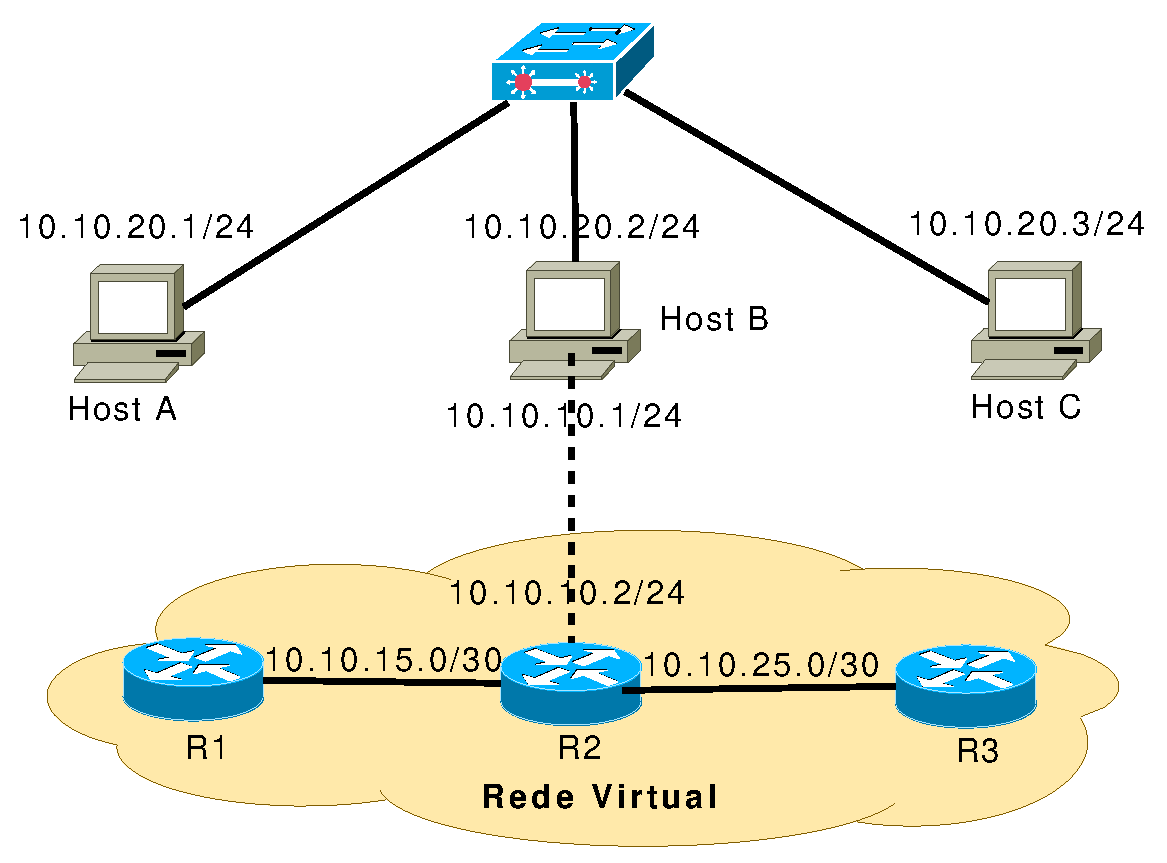
\includegraphics[scale=0.7]{ambiente_teste}
\caption{Ambiente de teste}
\label{fig:ambiente_teste}
\end{figure}

	Devido às dificuldades encontradas (ver capítulo \ref{cap:conclusao}), medições não puderam ser realizadas para que resultados fossem colhidos. Alguns testes foram realizados na medida do possível. Testes de integração foram realizados para verificar se os componentes do QoSPM estavam se comunicando corretamente.
	
	Para testar o QoSPM, nós utilizamos o laboratório localizado no módulo 2 do Lasid, pertencente ao projeto \textit{Um Modelo Híbrido e Adaptativo Tolerante à Falhas}. O laboratório é composto por três computadores e um \textit{switch} (Figura \ref{fig:ambiente_teste}), sendo que uma rede local (10.10.20.0) foi configurada com os três computadores.
	
	Existem três componentes QoSP executando na rede, um para cada \textit{host}. Além disso, existe um componente QoSPA executando no \textit{Host} B. O \textit{Host} B servirá tanto como hospedeiro para um QoSP como para um QoSPA, visto que não haviam máquinas suficientes. Além de hospedar os componentes citados anteriormente, o \textit{Host} B também passa a ser visto pelos componentes QoSP (inclusive pelo QoSP que executa em seu \textit{host}) como o roteador da rede. É importante salientar que o \textit{Host} B não se comporta como um roteador (visto que o mesmo não rotea pacotes e apenas uma rede local foi configurada). O \textit{Host} B é visto como roteador pelos QoSP para que os detectores de defeitos que executam nos mesmos possam ter um elemento a mais para monitorar.
	
	O roteador que havia sido adquirido para o projeto (um modelo 871 da Cisco) acabou não pudendo ser utilizado (para maiores detalhes ver capítulo \ref{cap:conclusao}). Para testar o monitoramento dos roteadores através do SNMP foi utilizado o Dynamips/Dynagen \cite{DYNAGEN08}. O Dynamips permite emular uma rede composta por roteadores Cisco, além de outros elementos de rede como \textit{switches}, em um computador. O Dynagen corresponde a um \textit{front-end} para o Dynamips, permitindo a configução de um laboratório de rede facilmente. Com a utilização do Dynamips foi possível criar uma rede virtual (Figura \ref{fig:ambiente_teste}) composta por três roteadores. O roteador R2 representa o roteador vinculado ao QoSPA, enquanto que R1 e R3 foram criados apenas para sobrecarregar R2. A rede virtual está "ligada" ao \textit{Host} B através de R2 (observe que a rede virtual está hospedada no \textit{Host} B e é vista apenas por ele), sendo que R2 era acessado através de uma interface virtual (10.10.10.1/30) criada com o \textit{tunctl}. O \textit{tunctl} é um comando utilizado para criar dispositivos TUN/TAP, sendo que estes dispositivos correspondem a \textit{drivers} que implementam dispositivos de rede através de \textit{software}, não necessitando de um adaptador de rede. TAP simula um dispositivo \textit{Ethernet} e opera na camada 2, enquanto o TUN simula um dispositivo da camada de rede e opera na camada 3. É importante salientar que o roteador virtual criado é visto apenas pelo QoSPA e serve apenas para testar o monitoramento executado pelo mesmo. Este roteador criado fornece funcionalidades semelhantes ao modelo 871 da Cisco, inclusive dando suporte à CISCO-CLASS-BASED-QOS-MIB.

	Para testar as funções \textit{QoS} e \textit{VerifyChannel} (ver capítulo \ref{cap:qos_provider}), um canal de comunicação foi definido, sendo este formado pelo processo $p_{x}$ que executa no \textit{Host} A, e $p_{y}$ que executa no \textit{Host} B. Os processos ficam trocando mensagens entre si periodicamente. A função \textit{VerifyChannel} foi executada no \textit{Host} C para verificar o estado do canal $c_{x/y}$, sendo assim, tanto a função \textit{VerifyChannel} como a própria função \textit{QoS} foram testadas. Os valores retornados pela função \textit{Delay} assim como o o intervalo de tempo durante o qual um canal deve ser investigado para verificar se houve tráfego foram configurados aleatoriamente, visto que o intuito era testar a integração entre os componentes.
	
	Para testar se a degradação era detectada, os roteadores R1 e R3 foram criados para sobrecarregar o roteador R2. R1 ficava enviando periodicamente mensagens \textit{ECHO REQUEST} para R3 enquanto que  R3 ficava enviando periodicamente mensagens do mesmo tipo no sentido inverso. Os pacotes ICMP (\textit{ECHO REQUEST}) foram configurados para receber o Serviço Expresso, sendo que este estava vinculado às interfaces 10.10.15.1 e 10.10.25.1 (na direção da saída) de R2. Quando o QoSPA requisitava informações da quantidade de pacotes descartados, sendo que esta requisição era feita no contexto da execução da função \textit{QoS}, o QoSPA percebia a degradação e notificava a degradação.
% !TEX encoding = UTF-8 Unicode
%\chapter{Conclusão}
\xchapter{Conclusão}{}
\label{cap:conclusao}
\acresetall
	
	O modelo proposto por \cite{GMCR07} mostrou-se inovador com relação ao fato de prover informações acerca dos estados dos processos em um sistema distribuído baseado na QoS disponível, sendo que o modelo adapta-se a esta QoS, permitindo que soluções eficientes sejam exploradas. Mas para que o modelo funcione corretamente, ele necessita gerenciar e acessar canais de comunicação com QoS. Este acesso é feito através do involúcro para arquiteturas de QoS denominado \textit{QoS Provider}. Mais especificadamente, o modelo HA necessita de informações da QoS dos canais de comunicação para que os estados dos processos em um sistema distribuído possam ser atualizados corretamente.
	
	Este trabalho visou a especificação e implementação do mecanismo de monitoramento do \textit{QoS Provider}, responsável por prover informações sobre a QoS dos canais de comunicação gerenciados pelo \textit{QoS Provider}. Procurou-se adotar princípios dos sistemas de monitoramento além de um modelo padrão para os sistemas de monitoramento.
	
	A especificação do QoSPM se deu através da modelagem do QoSPM, descrição do protocolo utilizado pelo mesmo e o desenvolvimento dos principais algoritmos que o compõe. Na modelagem utilizou-se a abordagem orientada a objetos e foi feita através da UML. Quando necessário, houve modelagem tanto do domínio como da aplicação. O protocolo descreveu as mensagens trocadas entre os componentes do QoSPM (QoSP, QoSPA e roteadores). As principais tarefas executadas pelo QoSPM foram especificadas através de algoritmos. Além da especificação, detalhes acerda da implementação foram abordados.
	
	Ainda com relação à especificação, uma arquitetura para o QoSPM foi especificada. A arquitetura do QoSPM é formada por dois componentes: módulos do QoSP e módulos do QoSPA. O QoSP é responsável por agregar informações referentes à QoS, sendo que estas foram colhidas junto aos roteadores pelos QoSPA, e também por detectar falhas dos componentes do QoSPM. No desenvolvimento da arquitetura, procurou-se adotar os princípios dos sistemas de monitoramento.
	
\section{Dificuldades encontradas}
	
	Inicialmente foram encontradas dificuldades com a configuração do ambiente, principalmente com relação à instalação do Xenomai. Cuidados com a configuração do arquivo do \textit{kernel} foram tomados para não comprometer a previsibilidade do Xenomai. Além disso, outro problema foi a falta do roteador que havia sido adquirido para o projeto. O roteador adquirido teve que ser devolvido visto que este não correspondia ao modelo que havia sido especificado e pelo qual havia sido pago, não sendo possível utilizá-lo para teste visto que não dava suporte ao \textit{Diffserv}. Até o presente momento da elaboração desta monografia, o modelo correto ainda não havia chegado. Tivemos também problemas com as placas de rede que dão suporte ao RTnet, visto que as mesmas só foram adquiridas há pouco tempo. Outro problema encontrado foi a não conclusão dos outros módulos do \textit{QoS Provider}, principalmente com relação ao módulo de cálculo do tempo de transmissão de mensagens em um canal de comunicação (corresponde à função \textit{Delay} do \textit{QoS Provider}). O detector de falhas que executa no componente QoSP do QoSPM necessita deste módulo para que os outros componentes do QoSPM possam ter suas falhas detectadas. A integração com o módulo de negociação não pôde ser realizada visto que este também não foi finalizado.
	
\section{Trabalhos futuros}

	Os trabalhos futuros estão relacionados com a integração do QoSPM com os outros módulos do \textit{QoS Provider}. A definição das estruturas de dados que devem ser compartilhadas entre os módulos assim como a forma como cada módulo deve utilizar a interface do outro faltam ser definidos. Testes completos devem ser realizados para que os resultados possam ser colhidos. Posteriormente à finalização do \textit{QoS Provider}, este último deve ser utilizado pelos algoritmos do modelo HA a fim de verificar, principalmente, se os tempos são satisfatórios para acessar as informações de QoS.


% Eh aconselhavel criar cada capitulo em um arquivo separado, digamos
% "capitulo1.tex", "capitulo2.tex", ... "capituloN.tex" e depois
% inclui-los com:
% \include{capitulo1}
% \include{capitulo2}
% ...
% \include{capituloN}
%
% Importante: 
% Use \xchapter{}{} ao inves de \chapter{}; se não quiser colocar texto antes do inicio do capitulo, use \xchapter{texto}{}.

%\xchapter{Introdu\c{c}\~{a}o}{Este eh o primeiro cap\'{\i}tulo, onde eu conto toda a historia deste trabalho, o problema, a solu\c{c}\~{a}o, etc.}
%
%% É recomendável utilizar `\acresetall' no início de cada capítulo para reiníciar o contator de referências às siglas.
%\acresetall 
%
%\section{Se\c{c}\~{a}o}
%Trabalho do  \ac{PGCOMP}. Bolsa do \ac{CNPq}.
%
%\begin{figure}[h]
%    Figure
%    \caption[As siglas também funcionam nas legendas]{As siglas também funcionam nas legendas, seja na forma de sigla \ac{CNPq}, seja na forma completa \acf{PGCOMP}.}
%\end{figure}
%
%\lipsum
%
%\subsection{Uma Subse\c{c}\~{a}o}
%\acresetall
%Texto para mostrar como o \verb|\acresetall| funciona \ac{CNPq}, \ac{PGCOMP}. Ele reseta os contadores e faz a sigla aparecer na forma estendida novamente.
%
%\subsection{Outra Subse\c{c}\~{a}o}
%
%Texto  \acf{CNPq}, \acf{PGCOMP}.
%
%
%\xchapter{Revis\~{a}o Bibliogr\'{a}fica}{Neste cap\'{\i}tulo eu apresento todo o material que eu estudei durante a elabora\c{c}\~{a}o do trabalho.}
%
%\lipsum
%
%Livro \cite{demeyer2008} e  livro \cite{raymond1999}.
%
%\xchapter{Exemplos}{} %sem preambulo
%
%A numera\c{c}\~{a}o de figuras \'{e} sequencial, dentro do cap\'{\i}tulo. Ver Figura \ref{default-regular1} e Figura \ref{default-regular2}.
%
%A numera\c{c}\~{a}o de tabelas \'{e} sequencial, dentro do cap\'{\i}tulo. Ver Tabela \ref{default-table1} e Tabela \ref{default-table2}.
%
%
%\section{Exemplos de Figura}
%
%\begin{figure}[htbp]
%\begin{center}
%  
\includegraphics[scale=0.5]{ufba.eps}
%\caption{Bras\~{a}o da UFBA - Menor.}
%\label{default-regular1}
%\end{center}
%\end{figure}
%
%\begin{figure}[htbp]
%\begin{center}
%  
\includegraphics[scale=0.75]{ufba.eps}
%\caption{Bras\~{a}o da UFBA - Maior.}
%\label{default-regular2}
%\end{center}
%\end{figure}
%
%\lipsum
%
%\section{Exemplos de Tabela}
%\subsection{Uma Tabela}
%\begin{table}[htbp]
%\caption{Uma tabela com 3 linhas e 2 colunas.}
%\begin{center}
%\begin{tabular}{|c|c|} 
%\hline
%elemento 11 & elemento 12 \\ \hline
%elemento 21 & elemento 22 \\ \hline
%elemento 31 & elemento 32 \\
%\hline
%\end{tabular}
%\end{center}
%\label{default-table1}
%\end{table}%
%
%\lipsum
%
%\begin{table}[htbp]
%\caption{Uma tabela com 3 linhas e 3 colunas.}
%\begin{center}
%\begin{tabular}{|l|c|c|} 
%\hline
%elemento 11 & elemento 12 & elemento 13\\ \hline
%elemento 21 & elemento 22 & elemento 23\\ \hline
%elemento 31 & elemento 32 & elemento 33\\
%\hline
%\end{tabular}
%\end{center}
%\label{default-table2}
%\end{table}%
%
%\xchapter{Outro cap\'{\i}tulo}{} %sem preambulo
%\lipsum


%% Parte pos-textual
\backmatter

% Bibliografia
% É aconselhável utilizar o BibTeX a partir de um arquivo, digamos "biblio.bib".
% Para ajuda na criação do arquivo .bib e utilização do BibTeX, recorra ao
% BibTeXpress em www.cin.ufpe.br/~paguso/bibtexpress
\bibliographystyle{abntex2-alf}
\bibliography{monografia}

% Apendices
% Comente se naoo houver apendices
\appendix

% !TEX encoding = UTF-8 Unicode
%\chapter{Entendendo os relacionamentos existentes na CISCO-CLASS-BASED-QOS-MIB}
\xchapter{Entendendo os relacionamentos existentes na CISCO-CLASS-BASED-QOS-MIB}{}
\label{apend:relacionamentos_MIB}
	
	Para entender as características de QoS relacionadas às classes configuradas nos roteadores Cisco, é necessário compreender alguns conceitos relacionados aos objetos de QoS e seus relacionamentos existentes na MIB \textit{CISCO-CLASS-BASED-QOS-MIB}. Objetos de QoS incluem mapas de classe (\textit{ClassMaps}), padrões de comparação (\textit{Match Statements}), mapas de políticas (\textit{PolicyMaps}) e ações (\textit{Feature Actions}).
	
\begin{itemize}
	\item \textbf{Match Statement}: Critérios de casamento de padrão para identificar pacotes com o propósito de classificação.
	
	\item \textbf{ClassMap}: A definição de uma classe que contém vários \textit{Match Statement} com o intuito de classificar pacotes em diversas categorias.
	
	\item \textbf{Feature Action}: Qualquer característica de QoS. Características de QoS incluem  declarações (regras) de policiamento, marcação, políticas de enfileiramento, entre outras. Depois que um pacote é classificado, ele pode ter uma ação aplicada ao mesmo.
	
	\item \textbf{PolicyMap}: Uma política definida para associar \textit{Feature Actions} às \textit{ClassMaps}. Para que os serviços de QoS (como o \textit{Diffserv}) possam ser oferecidos, uma \textit{PolicyMap} deve ser vinculada a uma interface lógica de um roteador. Neste caso, a política passa a ser chamada de \textit{Service Policy}.
\end{itemize}

	Cada objeto de QoS possui uma informação de configuração e uma informação estatística (de instância) relativa ao mesmo. Tais informações são armazenadas em tabelas e são acessadas através de índices. Estes dois tipos de informações se diferem nos seguintes aspectos:
	
\begin{itemize}
	\item \textbf{Informação de configuração}: Esta informação não muda mesmo se o objeto é vinculado à várias interfaces ou usado várias vezes. Ela é identificada unicamente para cada objeto com a mesma configuração através do índice \textit{cbQosConfigIndex}.
	
	\item \textbf{Informação de instância}: Esta informação muda à medida que o objeto é vinculado à várias interfaces ou utilizado várias vezes. Cada uso de um objeto de QoS corresponde a uma instância deste objeto. Cada instância de um objeto é identificada unicamente em um dispositivo (roteador) através do índice \textit{cbQosObjectsIndex}.
\end{itemize}

	Além dos índices citados anteriormente, outro índice importante nesta MIB é o \textit{cbQosPolicyIndex}. Este último é utilizado para identificar cada \textit{PolicyMap} adicionada a uma interface. Para cada interface na qual está adicionada, uma \textit{PolicyMap} terá um \textit{cbQosPolicyIndex} diferente. Como o foco principal na análise da QoS está em obter informações relativas às políticas (\textit{Service Policy}) e estas se relacionam com as outras características de QoS de forma hierárquica (para cada \textit{PolicyMap} existem uma ou mais declarações \textit{ClassMap}, sendo que para cada declaração \textit{ClassMap} existe uma ou mais \textit{Feature Action} associadas), os índices \textit{cbQosPolicyIndex} e \textit{cbQosObjectsIndex} são utilizados para identificar unicamente uma instância de objeto QoS do qual se interessa obter alguma informação. Cada vez que o roteador é reinicializado, os valores destes \textit{indexes} são diferentes (ou melhor, possivelmente não serão iguais)

	Todas as tabelas utilizadas na \textit{CISCO-CLASS-BASED-QOS-MIB} relacionadas com informações de configuração serão acessadas através do \textit{cbQosConfigIndex}, enquanto que para acessar as tabelas com informações estatísticas são necessários dois índice: \textit{cbQosPolicyIndex} e \textit{cbQosObjectsIndex}.
% !TEX encoding = UTF-8 Unicode
%\chapter{Descobrindo os índices para acessar informações estatísticas das classes na CISCO-CLASS-BASED-QOS-MIB}
\xchapter{Descobrindo os índices para acessar informações estatísticas das classes na CISCO-CLASS-BASED-QOS-MIB}{}
\label{apend:indices_MIB}
	
	Como foi dito no Apêndice A (é necessário ler o Apêndice A para compreender este), as tabelas com informações estatísticas necessitam dos índices \textit{cbQosPolicyIndex} e \textit{cbQosObjectsIndex} para serem acessadas. O monitoramento dos roteadores será no nível da classe e, para que se possa verificar se a QoS nas classes está sendo mantida, informações estatísticas relativas a estas necessitam ser colhidas. A seguir será descrito o procedimento necessário para descobrir os dois índices citados anteriormente relativos à classe do serviço Expresso configurada no roteador. Considere que a seguinte \textit{PolicyMap} está configurada no roteador com o intuito de tratar os fluxos dos canais \textit{TIMELY}:
	
\begin{tabbing}
Coma\=ndo 1: \\
\> clas\=s-map match-all premium \\
\> \> match ip dscp 46
\end{tabbing}	

\begin{tabbing}
Coma\=ndo 2: \= \\
\> poli\=cy-map HANDLE\_TIMELY \\
\> \> clas\=s premium \\
\> \> \> priority 500
\end{tabbing}			
			
	Estes comandos são utilizados para configurar o serviço expresso em um roteador Cisco. O primeiro comando é utilizado para classificar os pacotes que irão receber o serviço Expresso. Pacotes com o DSCP 46 receberão tal serviço. Observe que não foi mostrado como os pacotes foram marcados com este DSCP, caso eles realmente tenham sido marcados no roteador (isto está fora do escopo deste apêndice). O segundo comando configura uma política para tratar os pacotes que receberão o serviço Expresso. Tal política deve estar vinculada a uma interface (\textit{Service Policy}) para que o serviço possa ser oferecido. Esta política deve ser aplicada à saída da interface e, dependendo do sentido dos fluxos de tráfego e do número de redes que o rotedor interconecta, esta política deverá ser aplicada à várias interfaces. É importante salientar que os passos a seguir são utilizados para identificar os dois índices de interesse supondo que a política está sendo aplicada à apenas uma interface. Pequenas alterações necessitam ser feitas para levar em consideração mais de uma interface.
	
	Antes de descrever os passos, é necessário falar um pouco da MIB \textit{IP-MIB}. Ela é padronizada pelo IETF, sendo utilizada para gerenciar as implementações IP e ICMP nos elementos de rede. Esta MIB define o objeto MIB \textit{ipAddEntIfIndex} (cujo OID é 1.3.6.1.2.1.4.20.1.2) responsável por identificar unicamente uma interface em um elemento de rede. Este identificador é também conhecido como \textit{ifIndex}.
	
\begin{enumerate}

\item Obter o \textit{ifIndex} que identifica unicamente a interface na qual está vinculada a política \textit{HANDLE\_TIMELY}

Suponha que o IP de tal interface seja 10.10.10.2. Então, através do envio de uma mensagem \textit{SNMP\_GET} com o OID 1.3.6.1.2.1.4.20.1.2.10.10.10.2, nós conseguimos obter o \textit{index} desejado. Vamos supor que tenha sido 1.

\item Obter o \textit{cbQosPolicyIndex} da política \textit{HANDLE\_TIMELY} vinculada à interface em questão

Dado que nós temos o \textit{ifIndex} da interface de interesse, podemos descobrir as políticas vinculadas a esta interface através do objeto MIB \textit{cbQoSIfIndex} (1.3.6.1.4.1.9.9.166.1.1.1.1.4), definido na MIB \textit{CISCO-CLASS-BASED-QOS-MIB}. Este objeto faz parte de uma tabela (1.3.6.1.4.1.9.9.166.1.1.1) que descreve as interfaces e políticas vinculadas às mesmas. Tal objeto MIB retorna o \textit{ifIndex} da interface para uma dada política na qual está vinculada. Como nós não temos ainda o \textit{cbQosPolicyIndex} da política de interesse, vamos caminhar na árvore dos objetos MIB através do caminho identificado pelo OID 1.3.6.1.4.1.9.9.166.1.1.1.1.4 para descobrir todos os pares política-interface do roteador. Suponha que o resultado seja:

1.3.6.1.4.1.9.9.166.1.1.1.1.4.\underline{1043} = INTEGER: 1

1.3.6.1.4.1.9.9.166.1.1.1.1.4.\underline{1065} = INTEGER: 2

Observe que no retorno da consulta, foi adicionado um número (a porção sublinhada) ao OID cuja árvore foi caminhada. Este número é exatamente o \textit{cbQosPolicyIndex} que faltava para identificarmos a política. A segunda parte das igualdades identifica o \textit{ifIndex} da interface. Como sabemos que \textit{ifIndex} da interface em questão é 1, o \textit{cbQosPolicyIndex} da política que nos interessa é 1043. No exemplo mostrado, existe apenas uma política vinculada à interface de interesse, mas poderiam existir duas políticas vinculadas, uma à saída e outra à entrada. Neste caso precisaríamos executar o passo seguinte.

\item Descobrir o \textit{cbQoSPolicyIndex} da política vinculada à saída da interface

	Para executar este passo, vamos utilizar o objeto MIB \textit{cbQoSPolicyDirection} (cujo OID é 1.3.6.1.4.1.9.9.166.1.1.1.1.3), definido no mesmo contexto (tanto da MIB como da tabela) do objeto MIB utilizado no passo anterior. Tal objeto MIB indica a direção do tráfego para o qual a política será aplicada. Também vamos caminhar na árvore dos objetos MIB, mas neste caso através do caminho identificado pelo OID 1.3.6.1.4.1.9.9.166.1.1.1.1.3 para descobrir todos os pares política-direção do roteador. Suponha que em relação ao exemplo anterior, foram adicionadas políticas às entradas da interface, e que o resultado da caminhada seja:
	
1.3.6.1.4.1.9.9.166.1.1.1.1.3.\underline{1043} = INTEGER: 2

1.3.6.1.4.1.9.9.166.1.1.1.1.3.\underline{1044} = INTEGER: 1

1.3.6.1.4.1.9.9.166.1.1.1.1.3.\underline{1065} = INTEGER: 2

1.3.6.1.4.1.9.9.166.1.1.1.1.3.\underline{1066} = INTEGER: 1

A segunda parte das igualdades acima identifica o sentido do fluxo para o qual a política é aplicada. O valor 1 significa que a política é aplicada à entrada da interface, enquanto que o valor 2 significa o oposto. Se este mesmo exemplo se aplicasse ao passo anterior , nós estaríamos em dúvida (com relação ao \textit{cbQoSPolicyIndex}) entre 1043 e 1044, supondo que ambos se aplicassem à interface identificada pelo \textit{ifIndex} 1. Mas agora saberíamos que o \textit{cbQoSPolicyIndex} da política em questão aplicada à interface de interesse é 1043, visto que esta política está sendo aplicada à saída da interface.
		
\item Descobrir o \textit{cbQosConfigIndex} da classe premium

Para executar este passo, vamos utilizar o objeto MIB \textit{cbQoSCMName} (cujo OID é 1.3.6.1.4.1.9.9.166.1.7.1.1.1), também definido na MIB \textit{CISCO-CLASS-BASED-QOS-MIB}. Este objeto faz parte de uma tabela (1.3.6.1.4.1.9.9.166.1.7.1) que especifica informações de configuração das classes (\textit{ClassMap}). Tal objeto MIB retorna o nome da classe, identificada pelo \textit{cbQosConfigIndex}. Como nós não temos ainda este índice, vamos caminhar na árvore dos objetos MIB através do caminho identificado pelo OID 1.3.6.1.4.1.9.9.166.1.7.1.1.1 para descobrir todos os pares classe-nome\_da\_classe do roteador. Suponha que o resultado seja:

1.3.6.1.4.1.9.9.166.1.7.1.1.1.\underline{1025} = STRING: class-default

1.3.6.1.4.1.9.9.166.1.7.1.1.1.\underline{1029} = STRING: premium

Observe que no retorno da consulta, foi adicionado um número (a parte sublinhada) ao OID cuja árvore foi caminhada. Este número é exatamente o \textit{cbQosConfigIndex} que identifica as classes configuradas no roteador. A segunda parte da igualdada mostra os nomes das classes. Como o nome da classe que nos interessa é \textit{premium}, então sabemos que o \textit{cbQosConfigIndex} desta classe é 1029. Apesar de nós não termos configurado a classe \textit{best-effort} anteriormente, por padrão, todo roteador possui tal classe para classificar os pacotes que não foram agregados nas outras classes.

\item Descobrir o \textit{cbQosObjectsIndex} da classe premium configurada na política \textit{HANDLE\_TIMELY}, vinculada à interface em questão

Para executar este passo, vamos utilizar o objeto MIB \textit{cbQoSConfigIndex} (cujo OID é 1.3.6.1.4.1.9.9.166.1.5.1.1.2), também definido na MIB \textit{CISCO-CLASS-BASED-QOS-MIB}. Este objeto faz parte de uma tabela (1.3.6.1.4.1.9.9.166.1.5.1) responsável por especificar a hierarquia de todos os objetos de QoS. Tal objeto MIB retorna o \textit{cbQoSConfigIndex} para um dado objeto (identificado pelos índices \textit{cbQosPolicyIndex} e \textit{cbQosObjectsIndex}). Como nós já temos o \textit{cbQosPolicyIndex} da política que nos interessa (1043) mas não temos ainda o \textit{cbQosObjectsIndex} da classe \textit{premium} para esta política, vamos caminhar na árvore dos objetos MIB através do caminho identificado pelo OID 1.3.6.1.4.1.9.9.166.1.5.1.1.2.1043 para descobrir todos os pares objeto-index\_de\_configuracao. Suponha que o resultado seja:

1.3.6.1.4.1.9.9.166.1.5.1.1.2.1043.\underline{1043} = Gauge32: 1035

1.3.6.1.4.1.9.9.166.1.5.1.1.2.1043.\underline{1045} = Gauge32: 1029

1.3.6.1.4.1.9.9.166.1.5.1.1.2.1043.\underline{1047} = Gauge32: 1033

1.3.6.1.4.1.9.9.166.1.5.1.1.2.1043.\underline{1049} = Gauge32: 1037

1.3.6.1.4.1.9.9.166.1.5.1.1.2.1043.\underline{1051} = Gauge32: 1025

1.3.6.1.4.1.9.9.166.1.5.1.1.2.1043.\underline{1053} = Gauge32: 1027

Os valores adicionados aos OID correspondem aos \textit{cbQosObjectsIndex} dos objetos de QoS. A segunda parte da igualdada mostra os \textit{cbQoSConfigIndex}. Como o valor deste último para a classe que nos interessa é 1029, então sabemos que o \textit{cbQosObjectsIndex} desta classe para o \textit{Service Policy} em questão é 1045.
\end{enumerate}

	Através destes passos, nós conseguimos descobrir os dois índices necessários para acessar as informações estatísticas da classe que fornece o serviço Expresso (\textit{premium}). Estas informações estão armazenadas na tabela \textit{cbQoSCMStatsTable} (cujo OID é 1.3.6.1.4.1.9.9.166.1.15.1). É importante salientar que todos estes passos devem ser executados apenas uma vez, durante o período de inicialização do QoS \textit{Provider}. Caso o roteador seja reinicializado, o processo também deverá ser repetido, visto que os valores dos índices possivelmente serão diferentes.

%\xchapter{Exemplo de Ap\^endice}{Um preambulo.} %sem preambulo
%\lipsum
% Eh aconselhavel criar cada apendice em um arquivo separado, digamos
% "apendice1.tex", "apendice.tex", ... "apendiceM.tex" e depois
% inclui--los com:
% \include{apendice1}
% \include{apendice2}
% ...
% \include{apendiceM}

%% Fim do documento
\end{document}
%------------------------------------------------------------------------------------------%

